\documentclass[11pt, oneside]{report}   	% use "amsart" instead of "article" for AMSLaTeX format
\usepackage{geometry}                		% See geometry.pdf to learn the layout options. There are lots.
\geometry{letterpaper}                   		% ... or a4paper or a5paper or ... 
%\geometry{landscape}                		% Activate for for rotated page geometry
%\usepackage[parfill]{parskip}    		% Activate to begin paragraphs with an empty line rather than an indent
\usepackage{graphicx}				% Use pdf, png, jpg, or eps with pdflatex; use eps in DVI mode
								% TeX will automatically convert eps --> pdf in pdflatex		
\usepackage{amssymb}
\usepackage{amsmath}

% MARCOS PARAGRAPH SEPARATION:
\setlength{\parindent}{0px}
\setlength{\parskip}{1em}

% CVL
\usepackage{times}
\usepackage{graphicx}
\usepackage{listings}
\usepackage{color}
\usepackage{url}
\usepackage{amsmath}
\usepackage{soul}
\usepackage[multiple]{footmisc}

% TILEHEAT
\newcommand{\minisec}[1]{\vspace*{0.05cm}\noindent\textbf{#1.}}

\title{Declarative Multi-scale Data Abstraction and Serving of Spatial Datasets}
\author{Pimin Konstantin Kefaloukos}
%\date{}							% Activate to display a given date or no date

\begin{document}
\maketitle

\tableofcontents

% STUART: Identifying the problem and objectives
% 1) SAY WHAT YOU'RE GOING TO SAY
% 2) SAY IT
% 3) SAY WHAT YOU JUST SAID
\chapter{Introduction}

In this dissertation, we investigate two classes of queries and associated data systems, which are used for designing and serving geographical maps respectively. We investigate query models and systems for \emph{multi-scale spatial data abstraction} (MSDA). Furthermore, we investigage query models and systems for \emph{multi-scale spatial data retrieval} (MSDR).

MSDA queries and systems are in play when people \emph{design} new maps. We investigate the design of easy-to-use MSDA query languages and the implementation of scalable systems for executing MSDA queries.

MSDR queries and systems are in play when users \emph{request} maps online. We investigate the requirements for MSDR queries and the implementation of high availability and high performance systems for executing MSDR queries. 

%Case Study, P1 enables P2, Mention where related work is (which parts/chapters)

% Emphasise map production and map consumption
\section{Motivation}
% Opportunities for users
\emph{Pannable} and \emph{zoomable} geographical maps are important because they allows users to explore large repositories of information at different focal points and levels of abstraction. Furthermore, \emph{web-based} maps enable online users world-wide to gain spatial insights and make spatial decisions on the go. For example, journalists can enrich online articles with digital maps based on the constantly emerging datasets online. Such maps give readers spatial insight into news stories with geographical aspects: the location of troops in a war, the extent of a pollution incident, places worth traveling to, etc. As another example, tourists can use digital maps and location based services (LBS) on mobile devices while exploring an unfamiliar city. Such maps support decision making: finding near-by restaurants, shops, points of interest, etc. Zoomable web maps have have many use cases, e.g. in social media, real-estate, government, science, policing, warfare, health, education and environmental control.%Finally, real-estate agents can advertise new deals on geographical maps, which is of great interest to people looking to buy or sell homes in a particular area. % work with the examples

Paragraph that summarizes the challenges. Be consistent about the order of challenges and their order in the thesis in general.

% Challenge 1: too many users
One challenge is encountered during the serving of maps. Today, users of maps have the opportunity to engage maps anytime and anywhere, caused by advances in mobile technology and near-ubiquitous web access in many parts of the world. As a consequence, web-based maps have attracted millions of users who bombard the end-points of spatial data services with a crushing request workload around the clock -- especially during peak hours. To handle this workload there is a need for scalable system architectures for maps. %TODO: Explain the challenges presented to system engineers further... and give some examples.

% Challenge 2: big data
Another challenge is encounted during the production of maps. Everyday, a mass of spatial data is accumulating online~\cite{agrawal2012bigdata}. There is a clear need to visualize much of this data on maps for the reasons mentioned above. However, manually editing maps based on emerging big data is prohibitively time-consuming. Furthermore, relying on GIS specialists to handle the task is expensive at best. What is needed is efficient and effective methods that can be used by non-experts who must perform tasks such as \emph{data abstraction} (e.g. data selection and aggregation)~\cite{haunert2006landcover,schmid2013opensciencemap} and \emph{visual abstraction} (e.g. graphical expression)~\cite{jacques1967semiologie} in order to create useful multi-scale maps~\cite{stolte2003multiscale,weibel1999generalising}. 

A couple of paragraphs that mention what I do to address these challenges. 

%These processes are made much harder in the context of Big Data. Furthermore, these tasks generally involve either preprocessing~\cite{sarma2012fusiontables,kefaloukos2014declarative} or indexing~\cite{bereuter2013real,nutanong2012multiresolution} of the data, which also becomes harder for Big Data. TODO: Give some examples

\section{Overview of State-of-the-Art Online Multi-scale Maps}
\subsection{Spatial Indexing}
% vector tiles, r-trees, linearization
\subsection{Multi-scale Data Abstraction}

\section{Requirements for Online Multi-scale Maps}
\subsection{Map Design Objectives}
% toepfer, constant info dens. metrics
\subsection{System Objectives}
% high-availability (basically no down-time), high-performance, scalable
\subsection{Usability Objectives}
% non-expert usage, time-efficient, effective
\subsection{Case Study: Danish Geodata Agency}
% authoritative data. consistent data. high-availability. high-performance. standards. cost-effective.

\section{Research Gaps}
\subsection{Programmability}
\subsection{Moving code to data}
\subsection{Unified Model for Multi-scale Data Visualization}
\subsection{Scalability}
\subsection{Resource Optimization}

% abstraction: usable by non-experts, programmability, unifying data abstraction across domains (addressed by CVL2)
% Vector Tiles: prediction

\section{Contributions}
\subsection{Survey of Automatic Methods for Geographical Data Abstraction}
\subsection{Design of Declarative Languages for Multi-scale Selection of Relational Data}
\subsection{Compilers for Multi-scale Selection Languages}
\subsection{Prediction and Tile Selection for Geospatial Workloads}
\subsection{Publications}

\section{Structure of this Dissertation}

\part{Multi-scale Data Abstraction}
% !TEX root = ./thesis.tex
\chapter{Overview of Multi-scale Geospatial Data Abstraction}

\section{Introduction}
% mention grundreich

\section{Logical Operators}
% Copy from notex.tex, foerster, shea+mcmaster, weibel
\subsection{Selected Algorithms}

\section{Multi-scale Approaches}
% mention ladder and star approach
\subsection{Ladder Approach}
\subsection{Star Approach}

\section{Processing Methods}
% See Pia Bereuter and Nunatuang
\subsection{Online Processing}
% mention data structures

\subsection{Off-line Processing}
% mention data structures

\section{Conclusion}


% !TEX root = ./thesis.tex
\chapter{Declarative Cartography: In-Database Map Generalization of Geospatial Datasets}

Creating good maps is the challenge of map generalization. An important generalization method is selecting subsets of the data to be shown at different zoom-levels of a zoomable map, subject to a set of spatial constraints. Applying these constraints serves the dual purpose of increasing the information quality of the map and improving the performance of data transfer and rendering.
Unfortunately, with current tools, users must explicitly specify which objects to show at each zoom level of their map, while keeping their application constraints implicit. This paper introduces a novel declarative approach to map generalization based on a language called CVL, the Cartographic Visualization Language. In contrast to current tools, users declare application constraints and object importance in CVL, while leaving the selection of objects implicit. In order to compute an explicit selection of objects, CVL scripts are translated into an algorithmic search task. We show how this translation allows for reuse of existing algorithms from the optimization literature, while at the same time supporting fully pluggable, user-defined constraints and object weight functions. In addition, we show how to evaluate CVL entirely inside a relational database. The latter allows users to seamlessly integrate storage of geospatial data with its transformation into map visualizations. In a set of experiments with a variety of real-world data sets, we find that CVL produces generalizations in reasonable time for off-line processing; furthermore, the quality of the generalizations is high with respect to the chosen objective function.

\section{Introduction}

%\marcos{The introduction now reads a bit too generic, and a bit too rich in buzzwords (big data, crowd sourcing). What is the problem that is being addressed?}
%what's the situation

%- why do people need to do cartographic generalization?

%- how do people go about this task today?

%- what is the main related work, and why is it not enough?

%Map generalization has a long tradition spanning hundreds of years, and has rightly been considered as much an art as a science~\cite{rieger1993consensus}.
%\marcos{Not very clear what map generalization really means, now that the examples are completely gone.}
%\marcos{GST?}
%\martin{The new abstract and introduction looks good, but I think that the examples in the old abstract would work well in one of the paragraph below. I would also suggest that "precision" and "legibility" is defined and/or examplified.}

The goal of map generalization is to produce a map at a given scale that achieves the right balance between rendering performance and information quality for end users. For example, in a tourist attraction rating system, one needs to efficiently visualize important attractions, and constrain object proximity to allow space for user interaction. In a journalistic piece that maps traffic incidents, however, maintaining the underlying distribution of data is the most important aspect, but at the same time object density must be constrained to ensure high-performance data transfer and rendering.

%A benefit of data reduction in digital maps is that performance can improve vastly be reducing the amount of data that needs to be handled when rendering a portion of the map. In \emph{automated} map generalization the generalization process is performed either entirely or partially by algorithms on a computer.

Fully automatic generalization of digital maps~\cite{sarma2012fusiontables,nutanong2012multiresolution} is relevant in many areas such as social networks, factivism and data journalism~\cite{cohen2011journalism,bono,sankaranarayanan2009twitterstand}, where there is a constant need for visualizing new and often massive geospatial datasets. Automatic generalization includes both data reduction and graphical rendering~\cite{weibel1999generalising,gruenreich1985cag}. Increasingly, graphical rendering is deferred to map clients. This trend leaves the challenging problem of data reduction, i.e., selecting the right information to be displayed across zoom levels of the map, to the map service provider~\cite{gaffuri12vectortiles}. 

Both the performance and quality of a generalized map become important as the map gains a large audience. A map generalization solution handling data reduction in this context should be able to deal with big spatial datasets, consisting of both point and polygon records, should be usable by novice programmers, and should be able to finish processing quickly, e.g., in time for a tight news agency deadline. Ideally, such a system will allow users to control the important aspects of generalization solutions using logical and concise measures and reuse existing technology as much as possible, e.g., relational database technology.

Unfortunately, current approaches for data reduction in map generalization fall short in one or many of the above dimensions. Recent work has mostly considered only explicit rules or pre-set constraints for map generalization, resulting in solutions that are either too tedious~\cite{sld,mapnik}, or too restrictive for users~\cite{sarma2012fusiontables,nutanong2012multiresolution}. In addition, previous solutions have been poorly integrated with existing technology, resulting in scalability bottlenecks such as being restricted to the main memory capacity of a single node~\cite{sarma2012fusiontables}. 
 

Spatial data is often stored in a database with powerful spatial extensions installed, so a natural idea is to exploit the processing capabilities of the database to perform map generalization. In this work, we present a novel \emph{database-integrated} approach that is a complete solution to the data reduction problem in map generalization. All operations are performed entirely within the database process, and the result is a preprocessing of spatial records for fast execution of subsequent scale-parameterized queries~\cite{hilbert1891ueber}. Essentially, a number is assigned to each spatial record corresponding to the lowest zoom-level at which the record should be visible in a zoomable map, allowing for efficient indexing.

Using a \emph{declarative language}, we allow the user to concisely express spatial constraints and object importance, which are used to compute a multi-scale database from an input table of spatial data. This gives users a large amount of control over the map generalization process, while still being extremely concise, expressing a generalization with as little as four lines of code. 

We term our approach \emph{declarative cartography}, since it combines a declarative language for data reduction with a compilation procedure that results in efficient database programs to transform data for cartographic visualization.

%\marcos{Revise arguments wrt. related work + open-source?}
%\martin{The paragraph below belongs, I think, to the related work section. Alternatively, it can be shortened a bit here and the extended version given in the related work section.}
%
%We know of two recent papers which address the problem of data reduction problem~\cite{nutanong2012multiresolution,sarma2012fusiontables}. While both of these approaches provide good solutions to the data reduction problem with good running time, there are distinct and overlapping shortcomings to both of these which are not suffered by our approach.  Both of these approaches support only fixed constraints, while we allow a large class of constraints to be defined by the user. The first paper~\cite{sarma2012fusiontables} seems to indicate that the dataset must fit main memory and implies that data must be serialized in and out of the database for processing, none of which is true of our system. The other published approach~\cite{nutanong2012multiresolution} seems to require modifications to the database engine, which is not true of our system either. Neither of these previously published systems offer a language interface to users, but do imply a mechanism for parameterizing the fixed constraints. While~\cite{sarma2012fusiontables} show that there is at least mathematical support in their approach for several different objective functions, it is not clear how a user would actually express new objectives in a way that is understood by the system. Finally, users can take our implementation and start running it on their own infrastructure using only free, unmodified, open source software.

\vspace{5em}

In this paper, we make the following four contributions:
\begin{enumerate}
\item We present a declarative language, Cartographic Visualization Language (CVL, pronounced ``civil''), for generalizing spatial datasets. CVL is designed to be simple and concise to use for novice programmers. The CVL language was designed in collaboration with the Danish Geodata Agency and Grontmij in Denmark.\footnote{\url{http://www.gst.dk/English/}}\footnote{\url{http://grontmij.dk/}}

\item We convert the data reduction problem in map generalization to an instance of the well-known \emph{set multicover problem}~\cite{rajagopalan1998primal}, which makes constraints fully pluggable and allows reuse of well-known algorithms~\cite{rajagopalan1998primal,vazirani2001approximation}.

\item We show how to fully evaluate CVL inside the database; this enables us to reuse basic database technology for data management and scalability. While CVL is designed to compile to a variety of engines~\cite{Stonebraker:2010:PDBMSvsMapReduce}, we present here an implementation using a relational database engine with spatial extensions. The code for the project is available as open source through the project website.\footnote{\url{http://github.com/dmslab/declarativecartography}}

\item We present experimental results for a variety of real datasets. The results show that the proposed approach has good performance and produces high-quality map generalizations.
\end{enumerate}

In Section~\ref{sec:background}, we define the data reduction problem in map generalization as a selection problem. In Section~\ref{sec:cvl:language}, we introduce the CVL language. In Section~\ref{sec:optimizationmodel}, we formalize the selection problem as a combinatorial optimization problem based on a mapping to the set multicover problem, and we revisit algorithms for this problem in Section~\ref{sec:algorithms}. In Section~\ref{sec:implementation}, we discuss the compilation procedure that enables us to run CVL on a relational database backend. Experimental results are presented in Section~\ref{sec:experimental}, and finally related work is summarized in Section~\ref{sec:related}.


\section{Selection of Geospatial Data}
\label{sec:background}

In the \emph{selection problem}, we wish to select the subset of a geospatial dataset to be visualized on a map at a given scale. Below we define the basic components of the problem, and informally define the associated optimization problem.

\subsection{Geospatial records and weights}
\label{sec:records}

The dataset is assumed to consist of a set of \emph{geospatial records} drawn from a database table. The schema of a geospatial record consists of a \emph{geometry} field (e.g. a point, line or polygon), a \emph{unique ID} field and any number of additional textual and numeric fields, such as ``city name'' and ``population''.

Each record is assigned a \emph{user defined weight} using CVL (see Section~\ref{sec:cvl:language}). The weight models the importance of a record, with high weight corresponding to great importance. Any subset of records --- or all records for that matter --- may have the same weight. Therefore, the weights induce a partial order of the records.

\subsection{Zoom levels and map constraints}
\label{sec:constraints}
For zoomable maps, different subsets of the data should be selected for display at different scales or \emph{zoom levels}. Let the zoom-levels run from 1 (lowest scale) to $\mathcal{Z}$ (largest scale). On a given zoom level, the map is rendered at a certain pixel resolution. Thus, for a given zoom level, we know the distance in pixels between geospatial locations. This gives rise to two particularly important map constraints~\cite{harrie2007modelling} when selecting data for a given zoom level.

Firstly, the \emph{principle of constant information density} implies that the number of records that can be displayed within an area of a certain pixel size should be bounded~\cite{topfer1966principles}. Assume that we divide the complete map into cells (or tiles) of, say, 256 x 256 pixels. The \emph{visibility} constraint states that each cell can contain at most $K$ selected records, where $K$ is a user-defined parameter~\cite{sarma2012fusiontables}.

Secondly, records cannot be too close to each other in the map --- otherwise the user will not be able to clearly distinguish between them. The \emph{proximity} constraint states that every pair of visible records must be separated by at least $d$ pixels, where $d$ is a user defined parameter.

In addition to these constraints that must hold separately for each zoom level, there are constraints that must hold across zoom levels. A particularly important constraint is the \emph{zoom-consistency} constraint, which states that when a record is filtered out at a given scale, it should also be filtered out at all \emph{lower} scales~\cite{sarma2012fusiontables}. When a user zooms out on a map, records can only disappear --- not reappear.

Apart from the zoom-consistency constraint, CVL supports constraints based on \emph{simple measures} that are \emph{satisfiable by selection} (see Section~\ref{sec:cvl:language}). A simple measure is a function that maps a set of records to a scalar value. A constraint is violated if the measure exceeds a threshold. A constraint is satisfiable by selection if we can \emph{always} satisfy it by simply deleting an appropriate subset of the records. Both the visibility and proximity constraints respect these restrictions. However, we cannot model constraints that have complex measures or cannot be satisfied by using selection alone, such as \emph{topology} and \emph{spatial distribution} constraints. We leave these classes of constraints to future work.

\subsection{Conflicts}
\label{sec:conflicts}

Constraints such as visibility or proximity can be modeled using the notion of \emph{conflicts}. A conflict is a set of records that cannot all be selected without violating the constraint.

For the visibility constraint, there is a conflict generated for every cell that contains more than $K$ records. For the proximity constraint, there is a conflict generated for each pair of records that is less than $d$ pixels apart (see Figure~\ref{fig:proximity:conflict}). A record can be in several conflicts, which is the case for point $p$ in the example shown in the figure. A solution to the selection problem is \emph{feasible} if there are no conflicts.

\begin{figure}[htbp]
\begin{center}
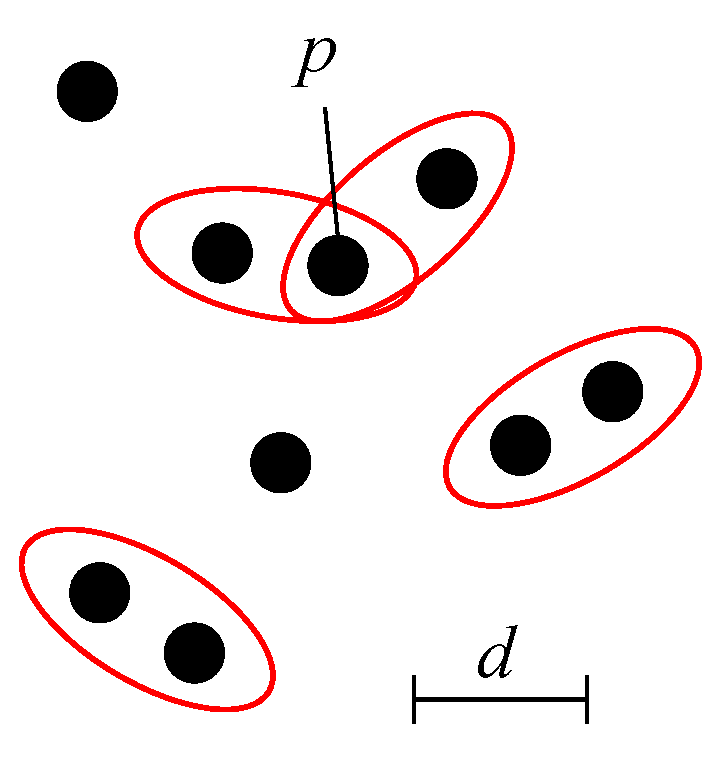
\includegraphics[scale=.3]{figs-cvl/cvl_proximity_conflicts.pdf}
\caption{Conflicts generated by the proximity constraint for distance $d$. Notice that point $p$ is a member of more than one conflict.}
\label{fig:proximity:conflict}
\end{center}
\vspace*{-4ex}
\end{figure}

Consider a conflict involving $k_1$ records, where at most $k_2$ of these records can be selected (where $k_1 > k_2$). Then it is equivalent to state that at least $\lambda = k_1 - k_2$ of these records must be \emph{deleted}. In the mathematical formulation of the problem in Section~\ref{sec:optimizationmodel}, we will use this alternative way to formulate conflicts.

\subsection{Selection as an optimization problem}
\label{sec:filtering}
The notion of conflicts is used to define the feasibility of solutions to the selection problem. This should be accompanied by a way to discriminate between solutions. Assigning an importance measure to each record, namely the record weights, intuitively allows us to measure the ``loss of importance'' due to records that are deleted.

In the optimization version of the problem, we seek the feasible solution that minimizes the aggregate weight of records that are deleted. In Section~\ref{sec:optimizationmodel}, we present a mathematical formulation of the selection optimization problem.

For a zoomable map with $\mathcal{Z}$ zoom levels, we are interested in finding $\mathcal{Z}$ solutions to the selection problem, one for each zoom level $i \in \{ 1, \ldots, \mathcal{Z} \}$. We call this problem the \emph{multi-scale selection problem}. To control the way in which we compute these solutions, we use an algorithmic framework known as the \emph{ladder} approach~\cite{foerster2010challenges}. This is a recursive approach, where the output of selection at large scale is used as input to selection at a smaller scale. This means that the zoom-consistency constraint (Section~\ref{sec:constraints}) is automatically satisfied.

The ladder approach is not appropriate for all use cases. For example, when regional labels are modeled as geospatial records, e.g., the label ``Europe'', we may wish to show a record only on intermediate zoom levels, violating zoom consistency. Handling these use cases would require an alternative formulation, e.g., following the \emph{star} approach~\cite{foerster2010challenges}. This is an interesting avenue for future work.  

% should be visible mostly on the intermediate zoom levels, the }\emph{star} approach~\cite{foerster2010challenges}\hl{ would be better. This is a limitation of the work presented in this paper.}

\section{CVL Language}
\label{sec:cvl:language}
The Cartographic Visualization Language (CVL) is a declarative language that can be used to specify an instance of the multi-scale selection problem (Section~\ref{sec:filtering}). CVL is a rule-based language with a similar goal as other rule-based languages for selection over spatial datasets, i.e., to control the density of information at each zoom-level~\cite{sld,mapnik}. The CVL approach is, however, markedly different. In the related languages, the user must explicitly control the selection of records at each zoom level, while also specifying how records are to be visualized. First of all, CVL focuses only on selection, not presentation. Furthermore, CVL controls selection in a novel constraint-based way. Instead of having the user explicitly control the selection of records at each zoom level, CVL lets the user choose \emph{map constraints} that are instead enforced at all zoom levels. By making the constraints explicit and the control implicit, a very concise formulation is obtained (see Figure~\ref{fig:cvl:example:airports} for an example).

CVL is one of the first languages and frameworks to implement the vision of reverse data management~\cite{meliou2011reverse}. In reverse data management, the core idea is that a user states a set of constraints and an objective. These are given together with an input database to an optimization algorithm which computes an output database that is feasible and optimal with regard to the constraints and objective (if a feasible solution exists). This is exactly how CVL works. Furthermore, a feasible solution is guaranteed to exist, as deleting all records is always a feasible solution.

The CVL language has two statements, the \emph{generalize} statement (see Section~\ref{sec:generalize:statement}) and the \emph{create-constraint} statement (see Section~\ref{sec:create:constraint:statement}). The create constraint statement is used to formulate new map constraints and the generalize statement is used to specify a solution to the multi-scale selection problem subject to those constraints. 

The CVL language builds on top of SQL and reuses SQL as a language for formulating constraints and record weighting schemes.

\begin{figure}[!t]
\begin{center}
\begin{lstlisting}
GENERALIZE 
   {input} TO {output}
WITH ID {expression}
WITH GEOMETRY {expression}
AT {integer} ZOOM LEVELS
WEIGH BY
  {float expression}
SUBJECT TO 
   {constraint} {float parameters} [AND
   {constraint} {float parameters} [AND
   ...]]
\end{lstlisting}
\vspace*{-1ex}
\caption{Syntax of generalize statement.}
\label{fig:generalize:syntax}
\end{center}
\vspace*{-4ex}
\end{figure}

\subsection{Generalize statement}
\label{sec:generalize:statement}

\begin{figure*}[tb]
  \begin{minipage}{0.329\linewidth}
    \centerline{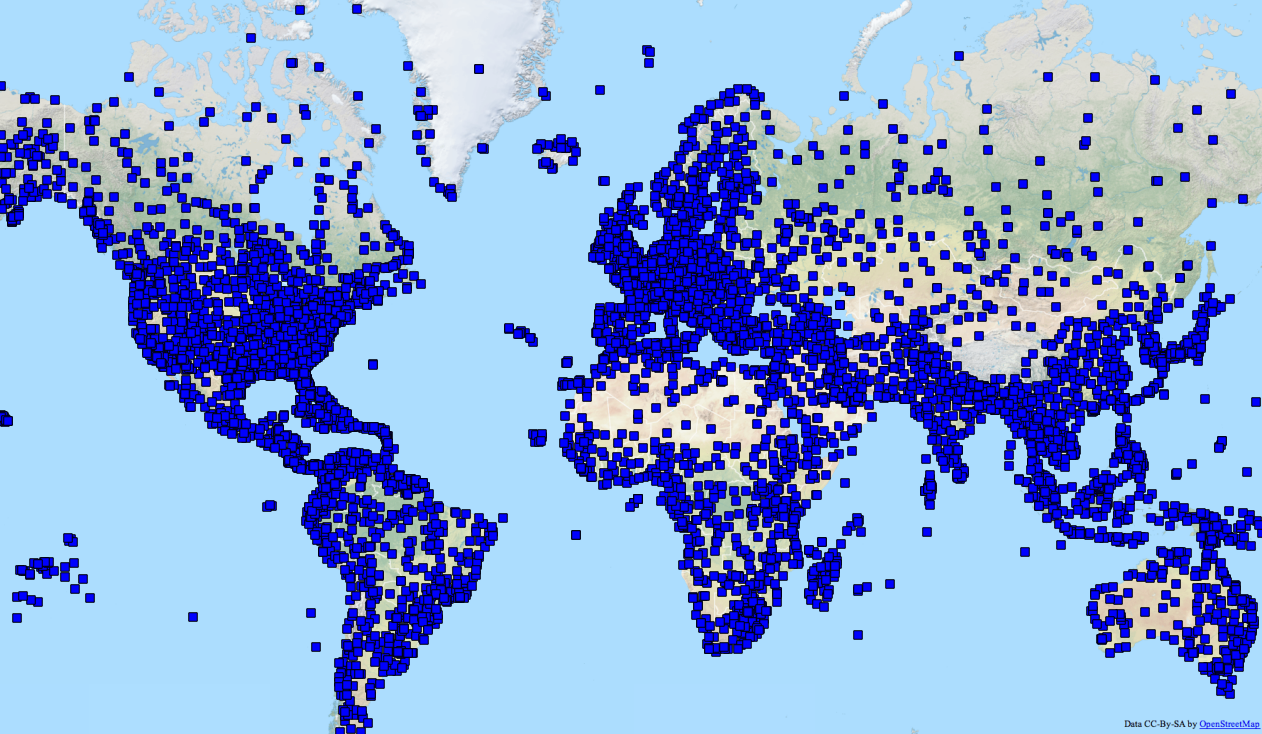
\includegraphics[width=0.95\linewidth]{figs-cvl/airports.png}}
    \centerline{(a) Full Openflights Airport dataset}
  \end{minipage} \hfill
  \begin{minipage}{0.329\linewidth}
    \centerline{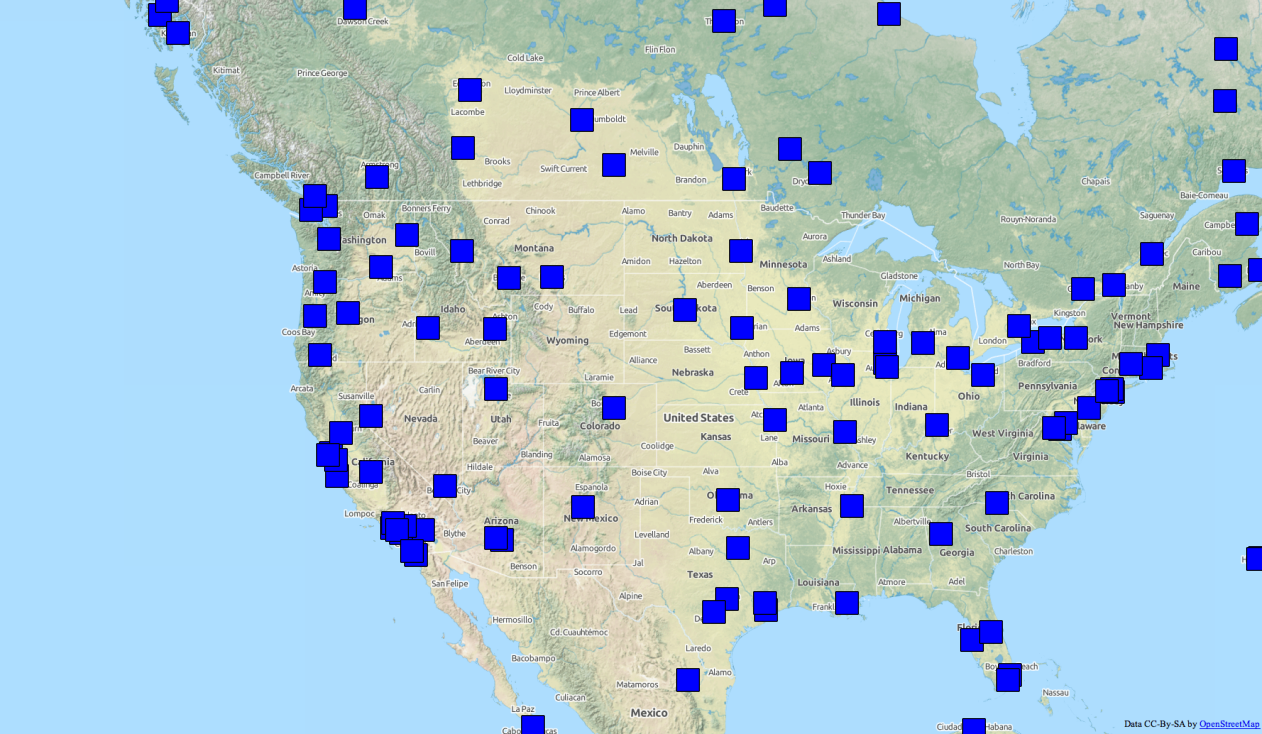
\includegraphics[width=0.95\linewidth]{figs-cvl/airports_z4.png}}
    \centerline{(b) Airports on zoom-level 5}
  \end{minipage} \hfill
  \begin{minipage}{0.329\linewidth}
    \centerline{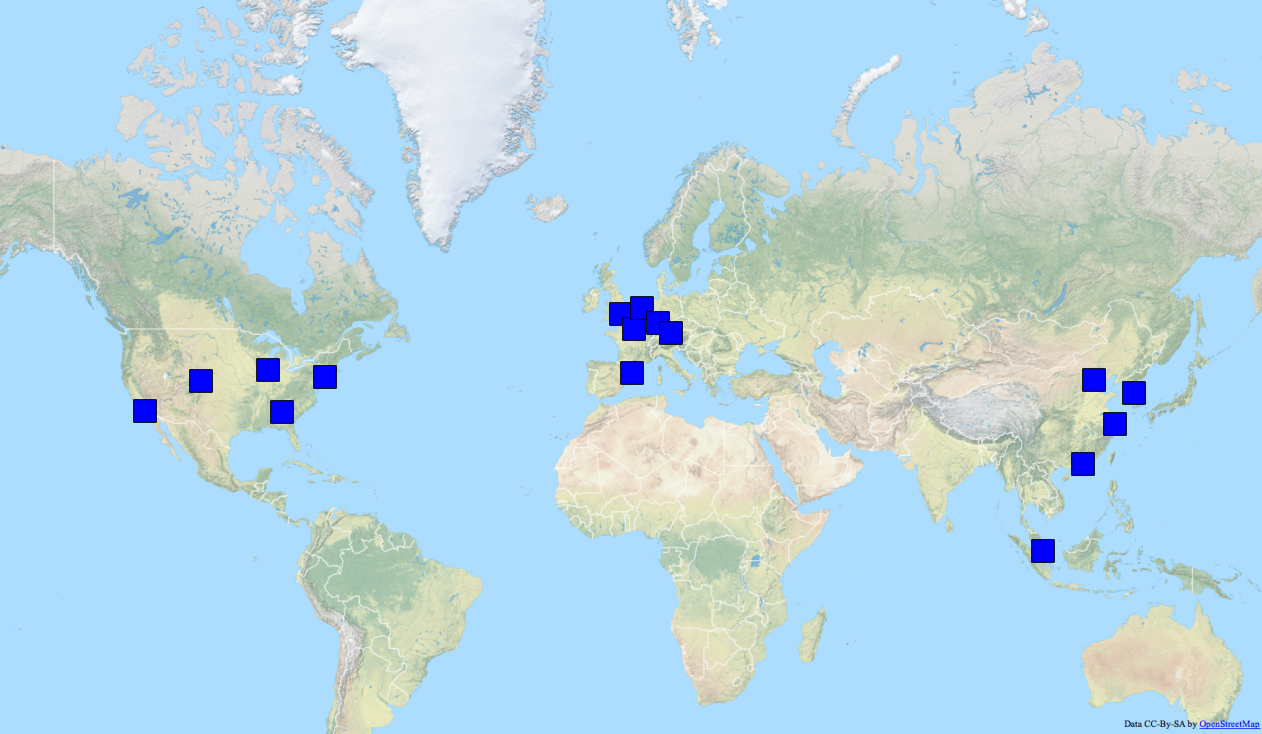
\includegraphics[width=0.95\linewidth]{figs-cvl/airports_z0.png}}
    \centerline{(c) Airports on the top-most zoom-level.}
  \end{minipage}
  \vspace{-0ex}
  \caption{Airport map (7K points) before (a) and after (b, c) running CVL. The output corresponds to the CVL statement in Figure~\ref{fig:cvl:example:airports}.}
  \label{fig:graphical:output:airport}
  \vspace{-2ex}
\end{figure*}

The generalize statement is the main statement in CVL. This statement creates a new multi-scale dataset from an input table of geospatial records, subject to user defined constraints. The syntax is shown in Figure~\ref{fig:generalize:syntax}. The statement has several clauses, beginning with the specification of input and output tables. Instead of giving the name of an input table, the user can optionally write a select statement in SQL of the form \texttt{(SELECT ...) t}. The next clause is the \emph{with-id} clause, which is used to uniquely identify records. If records have an id column, this clause could simply provide the name of that column. The \emph{with-geometry} clause is used to indicate the geometry property of records, e.g., the name of an available geometry column. The next clause is the \emph{zoom-levels} clause where the user writes a positive integer, which is the highest zoom level at which the selection process will begin. The \emph{weigh-by} clause is used to give an arbitrary floating point expression that is evaluated for each row in the input and used as weight for that record. The \emph{subject-to} clause lists the map constraints along with any parameters (as a comma-separated list). The \texttt{AND} keyword is used to separate constraints in the case more than one is used.

%For clarity the syntax is shown without two clauses, the \emph{with-id} clause and the \emph{with-geometry} clause, which are used simply to specify the names of the ID and geometry columns in the input table.


An example of generalizing a dataset using the generalize statement is shown in Figures~\ref{fig:graphical:output:airport} and~\ref{fig:cvl:example:airports}. In this example a dataset containing point records representing the location of airports world-wide is generalized (Figure~\ref{fig:graphical:output:airport}(a)). The records are weighted by using the name of a column containing the number of routes departing from each airport (shown in Figure~\ref{fig:cvl:example:airports}; CVL automatically handles the cast from integer to floating point). The intuition is that airports with more departures are more important. The single constraint that is enforced is the visibility constraint, with a parameter of $K=16$. Recall that the visibility constraint says that each tile can contain at most $K$ records.


\begin{figure}[h]
%\vspace*{-2ex}
\begin{center}
\begin{lstlisting}
GENERALIZE 
   airports TO airports2
WITH ID airport_id
WITH GEOMETRY wkb_geometry
AT 18 ZOOM LEVELS
WEIGH BY
  num_departures
SUBJECT TO 
   visibility 16 
\end{lstlisting}
\vspace*{-1ex}
\caption{Generalization of an airports dataset. The airports are weighted by number of departures. See Figure~\ref{fig:graphical:output:airport} for a vizualization of the result.}
\label{fig:cvl:example:airports}
\end{center}
\vspace*{-2ex}
\end{figure}



The resulting map is shown in Figure~\ref{fig:graphical:output:airport}(b) and~(c) and has at most $16$ airports on each tile. For the single tile on the top zoom-level, the world's sixteen busiest airports are shown. The CVL framework automatically gives priority to the airports with the highest weight. How this is done is explained in sections~\ref{sec:optimizationmodel} and~\ref{sec:algorithms}.

\subsection{Create constraint statement}
\label{sec:create:constraint:statement}

% change text
Map constraints are defined using the create-constraint statement.  The basic syntax of the statement is shown in Figure~\ref{fig:create:constraint:syntax}. The body of the statement is a SQL select statement that computes tuples that represent conflicts that are found at a given zoom level in the map. A tuple $\langle cid, rid\rangle$ denotes that record $rid$ is a member of conflict $cid$. See Section~\ref{sec:conflicts} for the exact semantics of conflicts.

\begin{figure}[h]
\begin{center}
\begin{lstlisting}
CREATE CONSTRAINT C1
AS NOT EXISTS
  {SQL select statement}
  
RESOLVE cid IF DELETE (
  {integer expression}
)
\end{lstlisting}
%\vspace*{-1.5ex}
\caption{Syntax of create constraint statement}
\label{fig:create:constraint:syntax}
\end{center}
\vspace*{-1ex}
\end{figure}

\begin{figure}[htbp]
\begin{center}
\begin{lstlisting}
CREATE CONSTRAINT Proximity
AS NOT EXISTS (
  SELECT 
    l.{rid} || r.{rid} AS cid,
    Unnest(array[l.{rid}, r.{rid}]) AS rid
  FROM
    {level_view} l
  JOIN
    {level_view} r
  ON
    l.{rid} < r.{rid}
  AND
    l.{geom} && ST_Expand(r.{geom}, 
      CVL_Resolution({z}, 256) * 
        {parameter_1})
  AND
    ST_Distance(l.{geom}, r.{geom}) <
      CVL_Resolution({z}, 256) * {parameter_1}
)

RESOLVE cid IF DELETE (
  1
)
\end{lstlisting}
%\vspace*{-2ex}
\caption{Definition of the proximity constraint.}
\label{fig:proximity:definition}
\end{center}
\vspace*{-1ex}
\end{figure}

The \emph{resolve-if-delete} clause is used to compute the integer number of records that must be deleted in order to resolve the conflict with a given $cid$. 
%\hl{For the proximity constraint, this number is always 1, but for other constraints this may vary}.

Using this syntax, the definition of the proximity constraint is given in Figure~\ref{fig:proximity:definition}. The body of the constraint is a distance self join using a distance function \texttt{ST\_Distance} provided by a spatial extension to SQL. This join finds all pairs of records that are too close, e.g.\ less than $10$ pixels apart. For each conflict, the select statement outputs two tuples and exactly once for each conflict. The resolve-if-delete clause is simply the constant $1$, because that is how many records must be deleted to resolve a proximity conflict.

In Figure~\ref{fig:proximity:definition}, some names are enclosed in curly braces, such as \texttt{\{rid\}}. These are variables which are bound at runtime by the CVL framework and are intended for making the definition of constraints simpler. The variables \texttt{\{rid\}} and \texttt{\{geom\}} are bound to the column names containing the ID and geometry of the records. The \texttt{\{level\_view\}} is bound to a view that contains all records that are visible at the current level, i.e., the records that have not been filtered out at a higher zoom-level. The function \texttt{CVL\_Resolution(\{z\}, 256)} is one of the utility functions defined by the CVL runtime, also with the purpose of making the definition of constraints simpler. This function returns the resolution (meter/pixel) at zoom-level \texttt{\{z\}}, where \texttt{\{z\}} is a variable bound to the currently evaluated zoom-level. The variable \texttt{\{parameter\_1\}} is the constraint parameter, e.g. $10$ pixels.

\begin{figure}[htbp]
\begin{center}
\begin{lstlisting}
CREATE CONSTRAINT Visibility
AS NOT EXISTS (
    SELECT
        busted_tiles.cid,
        busted_tiles.rid
    FROM
        busted_tiles
)

RESOLVE cid IF DELETE (
  SELECT count(*) - {parameter_1}
  FROM   busted_tiles bt
  WHERE  bt.cid = cid
)

WITH SETUP (
    CREATE TEMPORARY TABLE busted_tiles AS (
        SELECT
            t.cid,
            Unnest(array_agg(t.cvl_id)) AS rid
        FROM
        (
        SELECT
            CVL_PointHash(CVL_WebMercatorCells({geometry}, {z})) AS cid,
            {rid}
        FROM
            {level_view}
        ) t
        GROUP BY t.cid
        HAVING count(*) > {parameter_1}
    );
    CREATE INDEX busted_tiles_id_idx ON busted_tiles (cid);
)

WITH TEARDOWN (
  DROP TABLE busted_tiles;
)
\end{lstlisting}
%\vspace*{-1.5ex}
\caption{Definition of the visibility constraint.}
\label{fig:visibility:definition}
\end{center}
%\vspace*{-3ex}
\end{figure}



Figure~\ref{fig:visibility:definition} shows how the visibility constraint may be defined using CVL. The CVL definition uses an extension of the basic create-constraint syntax, namely the \emph{setup} and \emph{tear down} clauses. 
%which will be covered again in Section~\ref{sec:implementation:extensions}. 
The purpose of these clauses is to enable arbitrary SQL statements to be run before and after the constraint body is evaluated at each zoom-level. During the setup phase we create an auxiliary table called \texttt{busted\_tiles} which contains tuples $\langle tile\_id, rid \rangle$ identifying tiles that are intersected by more than $K$ records, and the ID of those records. The body of the constraint simply iterates over the auxiliary table, using the \texttt{tile\_id} column as the conflict ID.




The user does not need to know how the conflicts are handled, because all conflicts are automatically resolved by the CVL framework using one of the algorithms presented in Section~\ref{sec:algorithms}.

%In this example, calls are made to other CVL runtime functions, namely \texttt{CVL\_WebMercatorCells} and \texttt{CVL\_PointHash}. These functions returns a set of points corresponding to the centroids of intersected tiles (given a geometry) and a unique identifier for points, respectively. The unique identifier for points is based on the well-known GeoHash algorithm.


% give the variables by example, and explain together with the example, instead of listing everything up front.

%\marcos{These could be introduced by need along with the examples integrated into the sections above.}

\section{Selection optimization problem}
\label{sec:optimizationmodel}

In this section, we formally define the selection problem as an optimization problem. Let $R$ be the set of records in the dataset. Each record $r \in R$ has an associated weight $w_r > 0$ which models the importance of the record. 

Evaluating a CVL query generates a number of conflicts, i.e., all sets of records that violate a constraint. Let $C$ be the set of conflicts. A conflict $c \in C$ is a set of records $R_c \subseteq R$, where at least $\lambda_c \geq 1$ records must be deleted. The selection problem can now be modeled as a 0-1 integer program. Let $x_r$ be a 0-1 decision variable for each record $r \in R$ that is 1 if record $r$ is \emph{deleted}, and 0 otherwise. Then at a single-scale, the problem can be stated as follows:

\begin{align}
  \label{eq:objective}
  \min ~\sum_{r \in R} &w_r x_r \\
  \label{eq:general-constraints}
  \sum_{r \in R_c} x_r &\geq \lambda_c, ~~~~~~ c \in C \\
  x_r & \in \{0, 1\}, ~~ r \in R
\end{align}

The goal (\ref{eq:objective}) is to minimize the total weight of the records that are deleted. The inequalities (\ref{eq:general-constraints}) model the conflicts in the selection optimization problem. This is the \emph{set multicover problem} --- a generalization of the well-known set cover problem where each element needs to be covered multiple times instead of just once~\cite{rajagopalan1998primal}. In our formulation, conflicts correspond to \textit{elements} in the set multicover problem, while records correspond to \textit{sets}. Each conflict $c \in C$ must be ``covered'' $\lambda_c \geq 1$ times by choosing a subset of records that are deleted (i.e., for which $x_r=1$). Because the selection of records is modeled using a 0-1 decision variable, each record can be chosen at most once.

The general selection optimization problem is clearly equivalent to the set multicover problem. Since the set multicover problem is NP-hard, so is the general selection optimization problem. The selection optimization problem is even NP-hard for very restricted cases. Consider the vertex cover problem: Given a graph $G=(V,E)$, find a minimum size subset of the vertices $S$ such that every edge in $E$ has an endpoint in $S$. The vertex cover problem is equivalent to the restricted case of the selection optimization problem where all records have unit weight, and all constraints contain exactly two records. (The records are the vertices and the conflicts are the edges in the vertex cover problem.)

The vertex cover problem is NP-hard, even for very restricted cases. For example, if $G$ is a planar graph and every vertex has degree at most 3, the problem remains NP-hard~\cite{alimonti2000some, garey1977rectilinear}. This corresponds to a selection optimization problem where the conflicts contain two records each, and each record is involved in at most 3 conflicts. It is hard to imagine that any interesting application is more restrictive. 

In the next section, we discuss algorithmic approaches for solving the selection optimization problem. We include a further discussion on the objective value (\ref{eq:objective}) in the experimental evaluation of our approach.

\section{Algorithms for selection problem}
\label{sec:algorithms}

As mentioned in Section~\ref{sec:filtering}, we solve the multi-scale selection problem using the ladder approach. For each of the $\mathcal{Z}$ zoom levels, we generate and solve a separate instance of the selection optimization problem (Section~\ref{sec:optimizationmodel}). The solution gives us the records that should be deleted from zoom-level $i$. The remaining records are (conceptually) copied to zoom level $i-1$, unless we have reached the last zoom level ($i=1$). This approach is illustrated schematically in Figure~\ref{fig:algorithmic-framework}.

%\marcos{The algorithmic framework is not for multi-scale filtering, but for iterated single-scale filtering? Seems to me that these two are not the same thing.}
%\martin{Well, we do indeed solve (approximately) the multi-scale problem by iterated single-scale filtering, so I would say that this is okay. However, we don't have any good lower bound for the multi-scale problem, only for each of the single-scale problems.}

\begin{figure}[htbp]
\begin{center}
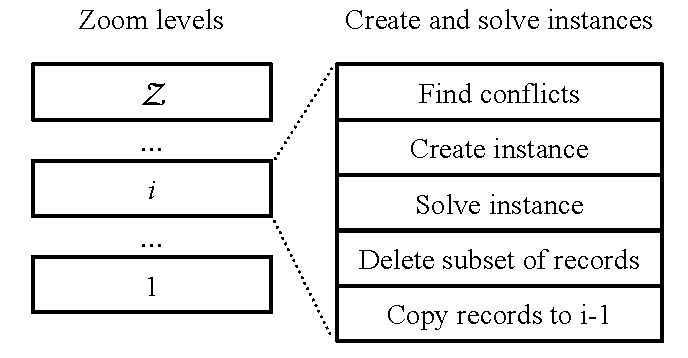
\includegraphics[scale=.6]{figs-cvl/cvl_stages.pdf}
\caption{Algorithmic framework: At each zoom level $i \in \{ 1, \ldots, \mathcal{Z} \}$ we solve a selection optimization problem. In the ladder approach, the problem is solved for the ``highest'' zoom level first.}
\label{fig:algorithmic-framework}
\end{center}
\end{figure}

Below we describe two different heuristic algorithms for solving the selection optimization problem. Let $n=|C|$ be the number of conflicts (or elements in the set multicover problem), and let $m=|R|$ be the number of records (or sets in the set multicover problem). Recall that $R_c \subseteq R$ is the set of records in conflict $c \in C$. The largest number of records in any conflict is $f = \max_{c \in C} |R_c|$, and is called the \emph{maximum frequency}.

\subsection{Static greedy algorithm (SGA)}
\label{sec:algorithms:sga}

In this algorithm, we consider each conflict $c \in C$ in turn, and simply choose the $\lambda_c$ records with minimum weight from the records $R_c$ --- independently of what has been chosen earlier. If the sets $R_c$ are disjoint, the algorithm is clearly optimal. However, in general no approximation guarantee can be provided. The algorithm runs in $O(n f \log f)$ time, as we just need to sort the records by weight for each conflict set; alternatively we can sort all records by weight in $O(m \log m)$ time and pick the minimum weight records from the conflicts in linear time in the total number of records in all conflict sets.

\subsection{LP-based greedy algorithm (LPGA)}
\label{sec:algorithms:lpga}

In this algorithm, we first solve a linear programming (LP) relaxation of the set multicover problem. This LP-problem is obtained by relaxing the constraint $x_r \in \{0, 1\}$ to $0 \leq x_r \leq 1$. Then we choose all records $r \in R$ for which the LP-solution variable $x_r$ is at least $1 / f$. Intuitively, we round up to 1 all fractional values that are large enough; the remaining fractional variables are rounded down to 0.

This algorithm provides a feasible solution to the selection optimization problem, and the approximation guarantee is $f$~\cite{vazirani2001approximation}; thus, if $f$ is small, the algorithm provides a good approximation guarantee. As the LP-problem can be solved in polynomial time, the complete algorithm is polynomial.

%\subsection{Dynamic greedy algorithm (DGA)}

%Described in Vazirani 13.2.1. @Martin: Please write here.

%\marcos{I would only introduce DGA if it is actually evaluated in the experiments.}

\section{Implementation}
\label{sec:implementation}

In this section, we describe how our implementation makes use of in-database execution to provide scalability and engine reuse for CVL (Section~\ref{sec:implementation:indatabase}). In addition, we discuss a number of extensions to CVL that we found to be useful for practical applications (Section~\ref{sec:implementation:extensions}). 

\subsection{In-Database Execution}
\label{sec:implementation:indatabase}

\minisec{Overview}
Since CVL is declarative, and CVL constraints are already expressed in SQL, it is natural to attempt to reuse as much existing DBMS technology as possible to execute CVL. Figure~\ref{fig:indatabase} shows how CVL is compiled for execution in a relational DBMS, which acts as the language runtime. The output of the CVL compiler is a database script for the target host, containing both SQL and stored procedures, and following the algorithmic framework of Figure~\ref{fig:algorithmic-framework}. The script is pushed down to the database engine, and operates against the appropriate input data stored in the system. This strategy offers us two main advantages:

\begin{enumerate}

\item Since all code is pushed down and both input and output reside in the database, we do not need to transfer any data outside of the database engine. This co-location of code and data is a significant advantage for large datasets.

\item By expressing as much as possible of the generated code in SQL, we can reuse decades of optimizations built into database engines, especially for geospatial data~\cite{Guttman1984:RTree,Hellerstein1995:GiST}. This opens up many opportunities, such as automatic optimization, parallelism, and selection of specialized algorithms and indexes.  

\end{enumerate} 

While the general strategy of compiling declarative languages to SQL has been pursued in other contexts, e.g., for XQuery~\cite{pathfinder} and LINQ~\cite{ferry}, our context poses a particular challenge of integrating the language with algorithmic solvers inside the database. 

\begin{figure}[htbp]
\begin{center}
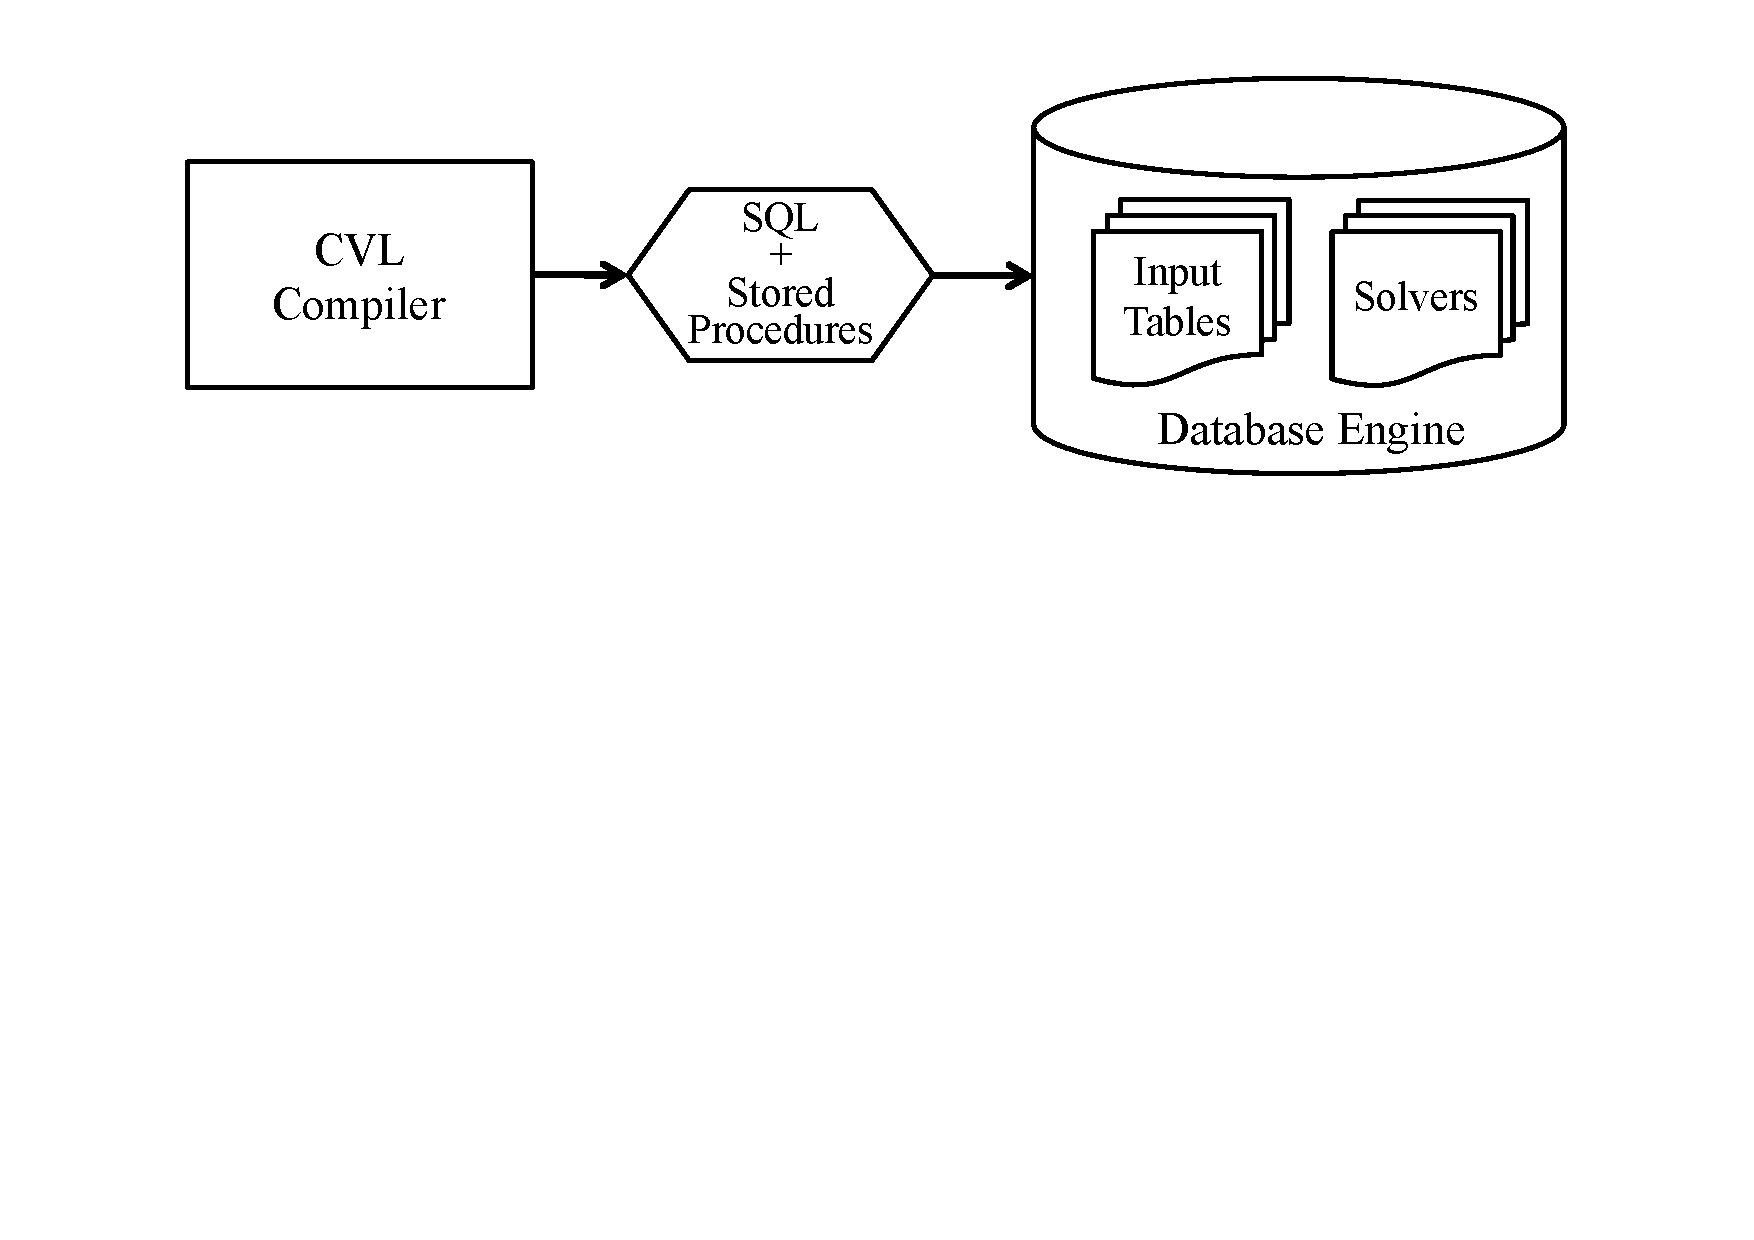
\includegraphics[scale=.35,viewport=400 375 450 550]{figs-cvl/indatabase-execution.pdf}
\caption{CVL and in-database execution.}
\label{fig:indatabase}
\end{center}
\vspace*{-1ex}
\end{figure}

\minisec{Solvers}
In Section~\ref{sec:algorithms}, we presented two different algorithmic approaches for solving CVL generalizations: static greedy (SGA) and LP-based greedy (LPGA). We now show how to express each of these approaches in SQL along with stored procedures. 

SGA is the simplest algorithm, and operates independently on the conflicts generated by each constraint. Suppose the conflicts $C$ generated by the active constraints are stored in a \emph{conflicts} table. Then SGA is tantamount to the query:

\begin{lstlisting}
SELECT rid
FROM (
  SELECT ROW_NUMBER() 
         OVER (PARTITION BY cid
               ORDER BY cvl_rank) AS r,
         rid, cvl_rank, lambda_c
  FROM conflicts) h
WHERE h.r <= h.lambda_c
\end{lstlisting}

For each conflict $c$, we order records by rank, and ensure that we pick at least $\lambda_c$ records. The declarative formulation allows us to reuse optimized sorting code in the database engine for execution.

LPGA solves a linear programming relaxation of the set multicover problem. We express LPGA by a stored procedure. The procedure accesses the conflicts for the constraints via SQL, constructs an appropriate LP, and then calls into an LP solver library. Since the solver library does not use built-in database optimizations, this execution strategy for LPGA only leverages the first advantage of data and code co-location listed above.

Finally, note that the code for finding conflicts is already expressed in SQL by the user for each constraint. As a consequence, this user code can make use of all built-in database optimizations available in the target engine.

\minisec{CVL runtime functions}
In the definition of the visibility constraint in Section~\ref{sec:create:constraint:statement}, we reference two stored procedures in the CVL runtime library, \texttt{CVL\_PointHash} and \texttt{CVL\_WebMercatorCells}. These functions are implemented in SQL and make use of the spatial extension of the database.

The procedure \texttt{CVL\_PointHash} uses a call to \texttt{ST\_GeoHash} to implement an injective mapping from points to strings. The GeoHash algorithm corresponds to a Z-order curve, and we exploit this for uniquely naming tiles when evaluating the visibility constraint, i.e. finding tiles with more than $K$ records.

The \texttt{CVL\_WebMercatorCells} function maps a geometry at a given zoom level to centroids of all intersected tiles (on that zoom level). We experimented with several ways to do this for general geometries (points, line segments, polygons) and found that rasterizing the geometry (using the function \texttt{ST\_AsRaster} in the spatial extension of the database) and iterating over the indices was the fastest for general geometries. For point records it is significantly faster to use the standard transformation function \texttt{ST\_SnapToGrid}.

%An improvement to \texttt{CVL\_WebMercatorCells} that we did not have time to implement is to compute tiles as quad-keys on the highest level only. Tile identifiers for lower levels are easily computed by taking prefixes of the quad-keys. This approach only benefits the running time when using constraints that are tile-based.

\subsection{Extensions}
\label{sec:implementation:extensions}

When designing CVL, we realized a number of interesting use cases for the language that we had not initially considered. This realization, along with our implementation experience of CVL use cases, led us to a set of extensions over the core language targeted at improving convenience of use. We present these extensions below.

\minisec{Partitioning and merging of datasets} 
A single input table may contain geospatial objects of different classes, e.g., roads and points of interest. When this is the case, users often wish to generalize some of these classes of objects independently, but obtain a single result map. While this can be done by merging the results of multiple GENERALIZE statements, we found it useful to add syntactic sugar to support this case. We extend the GENERALIZE statement with PARTITION BY and MERGE PARTITIONS clauses. PARTITION BY allows us to effectively segregate the input into multiple independent sets. MERGE PARTITIONS combines a few of these sets back together before providing them as input to generalization. For example, assume a \emph{geo\_objects} table contains highways, roads, restaurants, and hotels, tagged by a \emph{type} attribute. We could then generalize \emph{geo\_objects} as follows:

\begin{lstlisting}
GENERALIZE  geo_objects
TO network_and_poi_map
...
PARTITION BY type
MERGE PARTITIONS 'restaurant', 'hotel' 
              AS 'poi'
... 
\end{lstlisting}
\vspace{-1ex}

In the example, we overlay independent generalizations of highways, roads, and points of interest into a single map. However, restaurants and hotels are generalized as a single input set.  

\minisec{Forced and all-or-nothing visualization}
Intuitively, constraints let users specify what is \emph{not} allowed in a given map, by forbidding the existence of conflicts. However, users also find it helpful to control certain behaviors that \emph{must} occur in their map. We extended the GENERALIZE statement with support for two types of behaviors: (1)~the ability to mandate a minimum zoom level for a particular partition of the input, and (2)~the ability to force that either all or none of the objects of a given partition be displayed. For example, a user may wish to specify that highways must only appear at zoom level 10 or lower in their map. In addition, for topological consistency, either the whole highway skeleton is displayed or no highways should show up. To achieve this goal, we extend the GENERALIZE statement by a FORCE clause with MIN LEVEL and ALLORNOTHING specifiers. Continuing the example above:

\vspace{-1ex}
\begin{lstlisting}
...
FORCE MIN LEVEL 10 FOR 'highway' AND
ALLORNOTHING FOR 'roads'
... 
\end{lstlisting}
\vspace{-1ex}

In the evaluation of CVL, the minimum level specifier controls what data is given as input for a zoom level. The all-or-nothing specifier, on the other hand, controls filtering of the output of the level generalization process. If the specifier is present, all records of a partition are deleted if any record from the partition input is not present in the output. By filtering output, we ensure that the result also respects all other constraints specified by the user. 

%\minisec{Set up and Tear Down for Constraints}   
%Map constraints can exhibit significant complexity. Since a constraint is expressed as a single SELECT statement, it is often helpful to be able to refer to temporary tables in its formulation. We have thus extended the CREATE CONSTRAINT statement to include two additional clauses: WITH SETUP and WITH TEARDOWN. The former allows a user-defined SQL statement to be executed in advance of the constraint evaluation, creating any supporting tables for the evaluation of the constraint. The latter specifies user-defined cleanup code. Note that since constraints are evaluated independently at each zoom level, the set-up and tear-down clauses are evaluated before and after the constraint SQL at each zoom level.       
%\marcos{Move necessary information from paragraph above to Language section, and remove paragraph after that.}

%
% MVS: We can probably get away with not showing the syntax below. 
%
%\begin{lstlisting}
%CREATE CONSTRAINT C1 
%AS NOT EXISTS
% (SELECT cid, rid, minhits
%  FROM {more SQL})
%WITH SETUP
% {user-defined SQL}
%WITH CLEANUP
% {user-defined SQL}
%\end{lstlisting}

\section{Experimental Results}
\label{sec:experimental}

%\martin{Compare experimental results with theory e.g. expected approximation guarantee, number of constraints, number of records per constraint etc.}

In this section, we present experimental results with our implementation of CVL. Our experiments have the following goals:

\begin{itemize}

\item Evaluate the performance and solution quality of CVL generalizations with a variety of real-world datasets, including point data as well as complex shapes such as polygon and line data. 

\item Analyze the performance and solution quality of CVL generalizations produced under the proximity and visibility constraints presented in Section~\ref{sec:cvl:language} by both the SGA as well as the LPGA solvers of Section~\ref{sec:algorithms}.

\item Observe how the performance of CVL with different constraints and solvers scales with the number of objects in the geospatial dataset.

\end{itemize}

We start by presenting our experimental setup (Section~\ref{sec:exp:setup}), and then show results for both point data (Section~\ref{sec:exp:points}) and complex shapes (Section~\ref{sec:exp:complex:shapes}). Each result section discusses performance, quality, and scalability.


\subsection{Experimental Setup}
\label{sec:exp:setup}

\minisec{Datasets}
We have tested CVL using four real-world datasets, the largest of which containing 9 million points, and one synthetic dataset containing 30 million points. We list all datasets in Table~\ref{tab:datasets}. 

We have used three point datasets. The airports dataset is from Openflights and contains 7411 airports.\footnote{\url{http://openflights.org/data.html}} The tourism dataset contains 500 thousand points representing tourist attractions worldwide from the OpenStreetMap database.\footnote{\url{http://www.openstreetmap.org/}} The fractal dataset (synthetic) was created by iteratively copying and displacing points from the tourism dataset within a 10km radius until 30 million records were reached. We use this dataset for scalability experiments.

We have used two line datasets. The US rivers/streams dataset contains roughly 4 thousand rivers and roughly 27 thousand streams in the United States from the OpenStreetMap database. Records with identical name attributes have been merged into one. In the original dataset, most rivers are represented by multiple records, which is unfortunate in a selection situation (we wish to either select the waterway completely or not at all). 

We have used a single polygon dataset, the area information dataset from The Danish Natural Environment Portal, published by the Danish government.\footnote{\url{http://internet.miljoeportal.dk/}} This dataset contains 30 thousand high-fidelity administrative protection zone polygons, ranging from small polygons the size of buildings to large polygons the size of entire regions. The largest polygon has more than 36 thousand vertices.

%\minisec{Varying dataset size}
We have tested the scalability of CVL using both point and line datasets. A east-west unrolling approach is employed for gradually increasing the size of a dataset. First, we order records by x-coordinate, and then select increasingly larger prefixes of this order to derive larger datasets. The advantage of this approach over random sampling is that the spatial density of records is better preserved.

\begin{table}[htdp]
%\vspace{-2ex}
\caption{Datasets used in experiments}
%\vspace{-2ex}
\label{tab:datasets}
\begin{center}
\begin{tabular}{|c|c|c|c|c|}
\hline
\textbf{Origin} & \textbf{Dataset} & \textbf{Type} & \textbf{Records} & \textbf{Points} \\
\hline
Real & Airports & Points & $7K$ & $7K$ \\
Real & Tourism & Points & $500K$ & $500K$ \\
Synthetic & Fractal & Points & $30M$ & $30M$ \\
Real & US rivers & Line segments & $4K$ & $2M$ \\
Real & US rivers/streams & Line segments & $30K$ & $6M$ \\
Real & Proctection zones & Polygons & $30K$ & $9M$ \\
\hline
\end{tabular}
\end{center}
\label{default}
%\vspace{-2ex}
\end{table}%


\minisec{Hardware, software, and methods}
The machine used for testing was an Amazon EC2 instance with 17GB RAM, 2 x Intel(R) Xeon(R) CPU E5-2665 0 @ 2.40GHz and 20MB cache, running Amazon Linux 3.4.48-45.46.amzn1.x86\_64.\footnote{An image of the instance we used for testing is available through Amazon EC2 as an AMI. More information is available on the website for the project.}

The database used for testing was PostgreSQL 9.2.4 with PostGIS  2.0 built against the libraries GDAL 1.9.2 and GEOS 3.3.8. For the LP solver, we integrated the database with the convex optimization library CVXOPT version 1.1.6.\footnote{\url{http://cvxopt.org/}} We installed Python language bindings in the database against Python 2.6.8.

We ran each test three times on this installation, taking averages. We observed that measurements were very stable, with negligible difference in compute time between runs.

PostgreSQL always uses a single core to compute a transaction. Because the generalization process in CVL runs as a single long transaction, each job in CVL runs on a single core. A future direction would be to investigate parallel execution of CVL queries using a different language runtime such as a parallel database or a MapReduce environment.

\minisec{Average optimality ratio}
In our approach, we solve the multi-scale selection problem as a series of selection optimization problems. To get an indication of the solution quality, we compute for every selection optimization problem a lower bound using an LP-relaxation of the integer program. The numbers we present in Table~\ref{tab:points:overview} and Table~\ref{tab:complex:overview} include the average ratio between our solution value and the corresponding lower bound.


\begin{figure*}[tb]
  \begin{minipage}{0.329\linewidth}
    \centerline{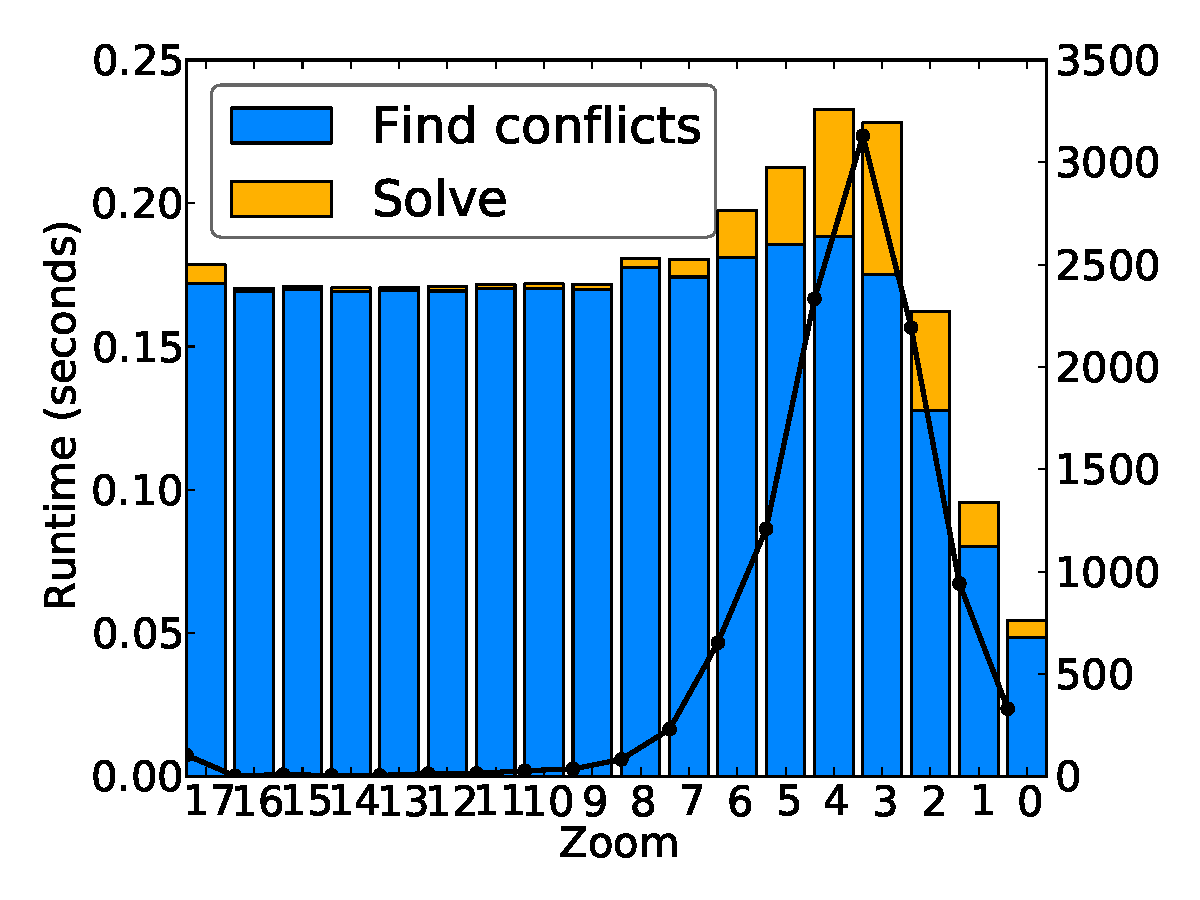
\includegraphics[width=0.9\linewidth]{figs-cvl/prelim_pnt_7k_airports_heuristic_B.pdf}}
    \centerline{(a) SGA + Proximity}
  \end{minipage} \hfill
  \begin{minipage}{0.329\linewidth}
    \centerline{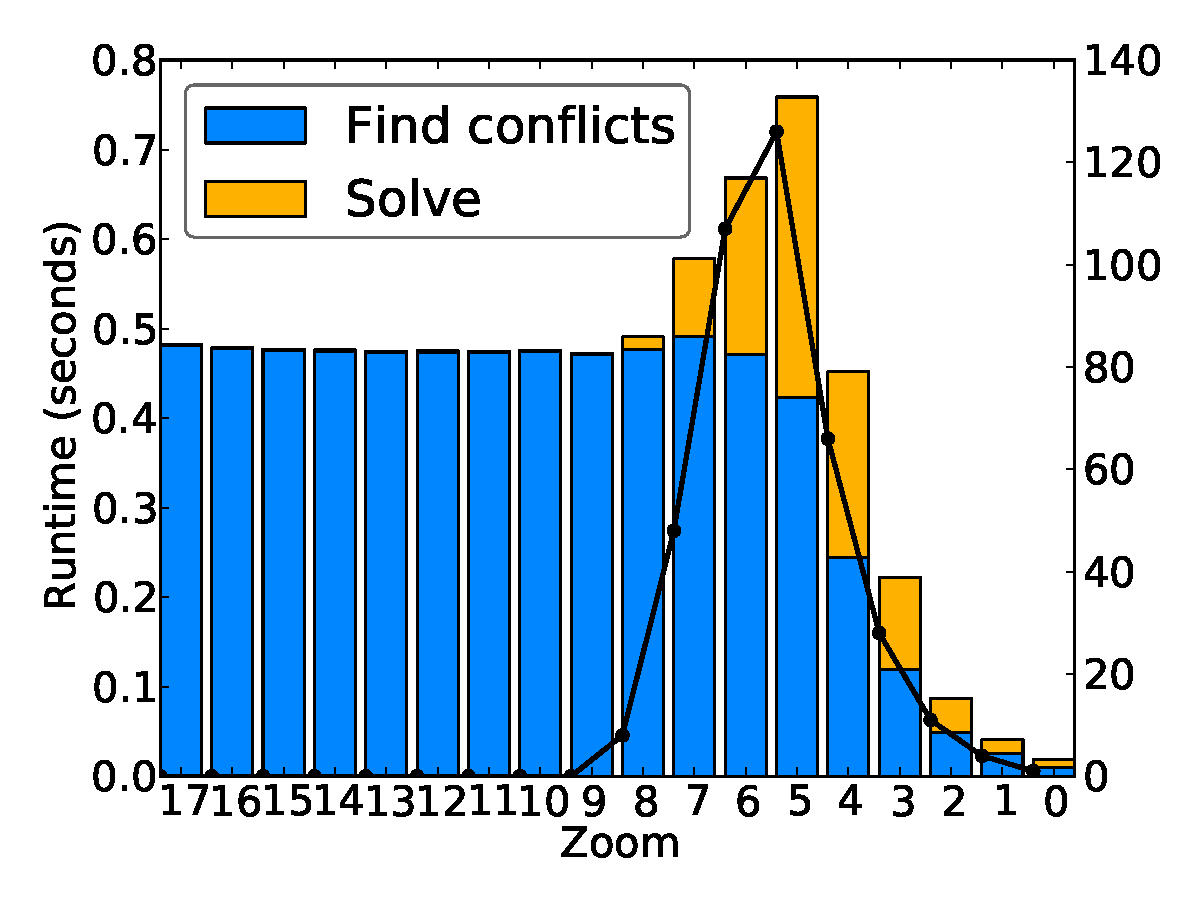
\includegraphics[width=0.9\linewidth]{figs-cvl/prelim_pnt_7k_airports_lp_A.pdf}}
    \centerline{(b) LPGA + Visibility}
  \end{minipage} \hfill
  \begin{minipage}{0.329\linewidth}
    \centerline{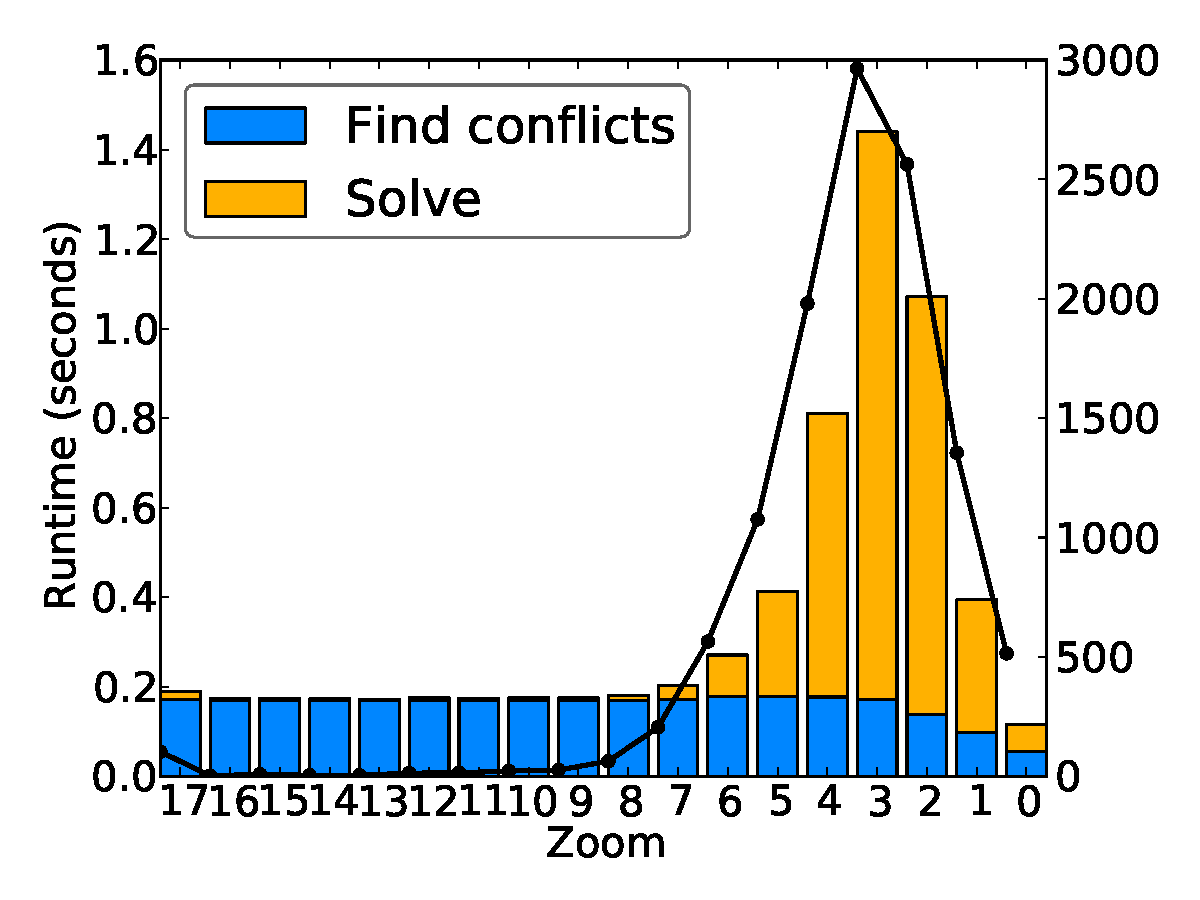
\includegraphics[width=0.9\linewidth]{figs-cvl/prelim_pnt_7k_airports_lp_B.pdf}}
    \centerline{(c) LPGA + Proximity}
  \end{minipage}
%  \vspace{-1ex}
  \caption{Performance breakdown by zoom level, Airport dataset (7K points). The black line indicates number of conflicts} \label{fig:performance:airport}
%  \vspace{-2ex}
\end{figure*}

\subsection{Point Data}
\label{sec:exp:points}

In this section, we present experimental results with point datasets, namely the Openflight airports and the tourism datasets. We first discuss performance and quality for CVL and then proceed to analyze CVL's scalability behavior. Even though we experimented with all combinations of solvers (SGA / LPGA) and constraints (visibility / proximity / combined), we show only representative results for brevity. Results for the combined visibility and proximity constraints exhibited the same performance trends as of the most expensive of the two constraints. All other results followed similar trends as the ones explored below.



\begin{figure*}[tb]
  \begin{minipage}{0.329\linewidth}
    \centerline{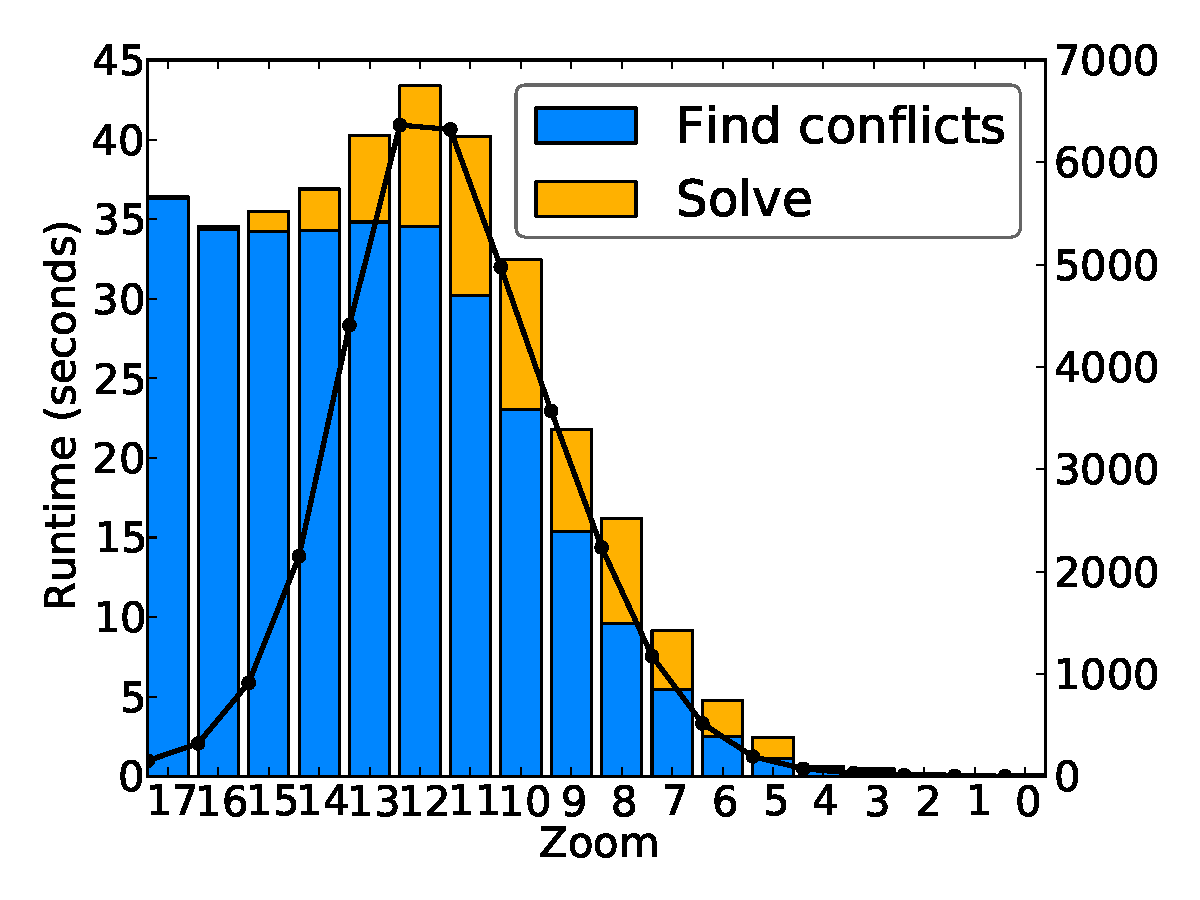
\includegraphics[width=0.9\linewidth]{figs-cvl/prelim_pnt_500k_tourism_heuristic_A.pdf}}
    \centerline{(a) SGA + Visibility}
  \end{minipage} \hfill
  \begin{minipage}{0.329\linewidth}
    \centerline{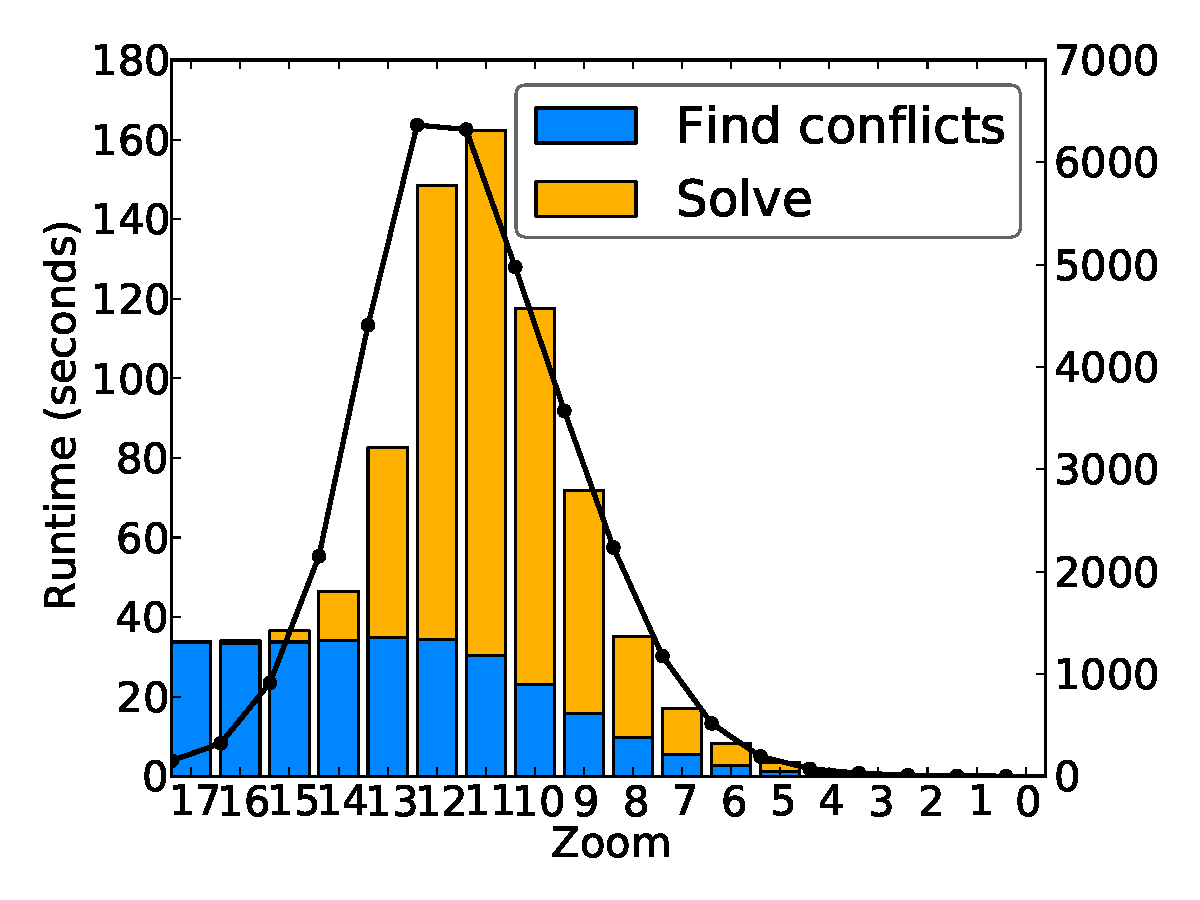
\includegraphics[width=0.9\linewidth]{figs-cvl/prelim_pnt_500k_tourism_lp_A.pdf}}
    \centerline{(b) LPGA + Visibility}
  \end{minipage} \hfill
  \begin{minipage}{0.329\linewidth}
    \centerline{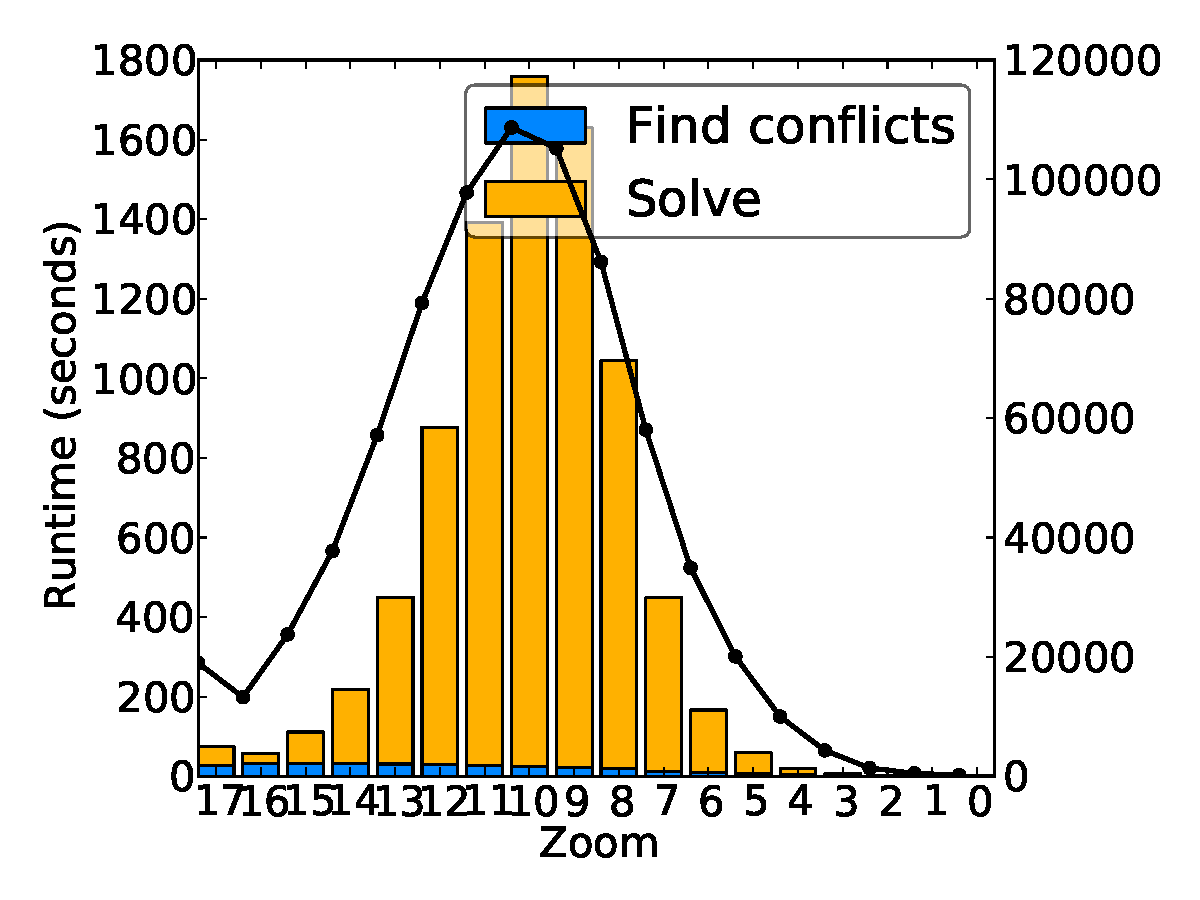
\includegraphics[width=0.9\linewidth]{figs-cvl/prelim_pnt_500k_tourism_lp_B.pdf}}
    \centerline{(c) LPGA + Proximity}
  \end{minipage}
%  \vspace{-1ex}
  \caption{Performance breakdown by zoom level, Tourism dataset (500K points). The black line indicates number of conflicts} \label{fig:performance:tourism}
\vspace{-1ex}
\end{figure*}

\minisec{Overall performance and quality}
An overview of running times and solution qualities for the point datasets are shown in Table~\ref{tab:points:overview}. In Section~\ref{sec:algorithms:sga}, we remarked that SGA is optimal for disjoint conflict sets. This is confirmed by the entries for visibility + SGA in the table. For the point datasets we used for testing, the LPGA algorithm is also optimal or within $3\%$ of the optimum when combined with the visibility constraint, likely caused by the conflict sets being disjoint. Recall that the approximation guarantee of LPGA is $f$ (see Section~\ref{sec:algorithms:lpga}).

In terms of quality, the difference between SGA and LPGA is not stark for either constraint. The difference depends more on the constraint than on the solver, with visibility generally yielding the best solutions. However, the running time of SGA can be substantially shorter than that of LPGA. We analyze this effect in the following.

\begin{table}[htdp]
%\vspace{1ex}
\caption{Results for CVL on point datasets grouped by constraint}
%\vspace{-2ex}
\begin{center}
\begin{tabular}{|c|c|c|c|c|}
\hline
\textbf{Dataset} & \textbf{Constraint} & \textbf{Solver} & \textbf{Time} & \textbf{Avg. opt. ratio}\\ 
\hline
Airports (7K) & Visibility & SGA & 7s & 1.0 \\
Airports (7K) & Visibility & LPGA & 7s & 1.03 \\
Tourism (500K) & Visibility & SGA & 6m 9s & 1.0 \\
Tourism (500K) & Visibility & LPGA & 13m 35s & 1.0 \\
\hline
Airports (7K)  & Proximity  & SGA & 3s & 1.18 \\
Airports (7K)  & Proximity & LPGA & 7s s & 1.22 \\
Tourism (500K) & Proximity & SGA & 7m 17s & 1.21 \\
Tourism (500K) & Proximity & LPGA & 2h 18m & 1.24 \\
\hline
\end{tabular}
\end{center}
\label{tab:points:overview}
%\vspace{-2ex}
\end{table}%

\begin{figure*}[tb]
  \begin{minipage}{0.49\linewidth}
    \centerline{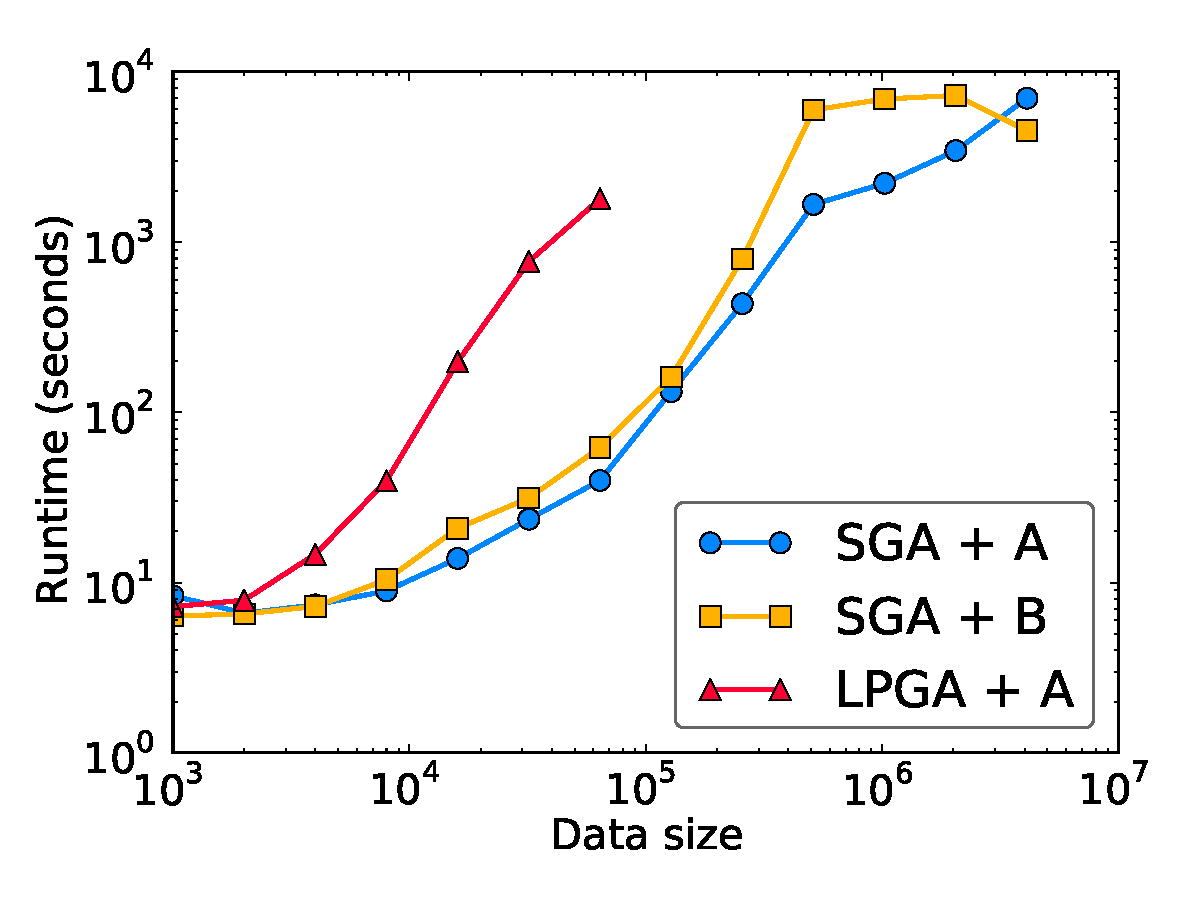
\includegraphics[width=0.75\linewidth]{figs-cvl/scal_pnt_30m_synthetic.pdf}}
    \centerline{(a) Scalability for point data}
  \end{minipage} \hfill
  \begin{minipage}{0.49\linewidth}
    \centerline{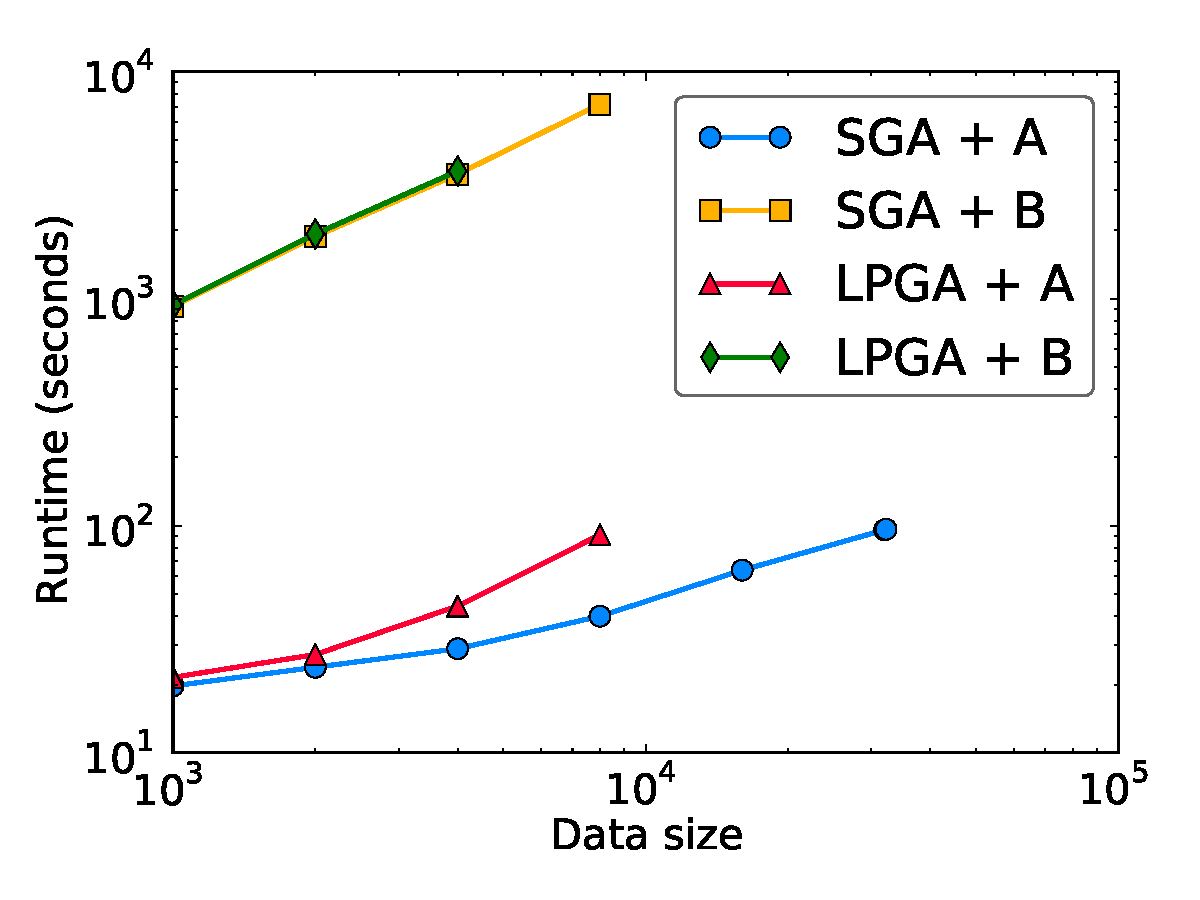
\includegraphics[width=0.75\linewidth]{figs-cvl/scal_lin_30k_uswaterway.pdf}}
    \centerline{(b) Scalability for complex shape data}
  \end{minipage} \hfill
%  \vspace{-0ex}
  \caption{Scalability of CVL for point datasets and complex shape datasets. Constraints are marked as \emph{Visibility}: A, \emph{Proximity}: B} \label{fig:scalability}
%\vspace{-1ex}
\end{figure*}

\minisec{Performance breakdown}
Figure~\ref{fig:performance:airport} shows the performance breakdown per zoom level of executing CVL with the Openflight airports dataset. Note the different y-scales in the graphs. We have overlayed the number of conflicts per zoom-levels as a black line. In Parts~(a)-(c), we observe that the time needed to find conflicts is roughly stable until eight zoom levels, then slightly increases, and finally drops sharply for lower zoom levels. The constraints used generate few conflicts at higher zoom levels, given the relatively low density of the airport distribution in space. Nevertheless, even though almost no conflicts are generated, the dataset is still processed, resulting in roughly equal time for finding conflicts and negligible time for solving conflicts per zoom level. 
 
As zoom levels decrease, more conflicts naturally arise, leading initially to increased conflict finding time, as well as conflict solving time. However, as conflicts are solved, records are deleted from the dataset taken as input for the next zoom level. This procedure causes conflict finding time (and eventually total time) to drop significantly for low zoom levels. For SGA under the proximity constraint (Part (a)), total time at zoom level zero is over two times shorter than the initial runtime at zoom level 17; for LPGA under the visibility constraint (Part (b)), the difference in total time reaches over an order of magnitude.  

Conflict solving time does not increase equally for different solvers. SGA exhibits conflict solving time that is consistently smaller than LPGA. Peak total time for SGA under the proximity constraint (Part (a)) is roughly four times shorter than for LPGA (Part (c)). In addition, LPGA is extremely sensitive to the number of conflicts reported by user-defined constraints. From Parts (b) and (c), we can see that LPGA exhibits peak conflict solving time over three times larger for the proximity constraint than for the visibility constraint, since the latter generates far fewer conflicts than the former.

Figure~\ref{fig:performance:tourism} exhibits results with the larger tourism attraction dataset. Since the dataset is denser in space than the airport dataset, conflicts are found and solved at higher zoom levels, resulting in an earlier drop in total time per zoom level. For Parts (a)-(c), total time is uninteresting for zoom levels lower than five. The same cannot be said, however, about peak total time in general, and about conflict solving time in particular.

Parts (a) and (b) compare performance of SGA and LPGA under the visibility constraint. Even though visibility generates a smaller number of conflicts than proximity, peak total time for LPGA is still roughly a factor of four larger than for SGA (see zoom level 11). Note that the difference is completely due to the efficiency of the solver, since the time to find conflicts is essentially the same for both methods. Total time for LPGA rises prohibitively when we employ the proximity constraint, reaching a baffling peak of near half an hour at zoom level 10 (Part (c)). While not shown, total times per zoom level for SGA under the proximity constraint are roughly comparable to the times reported in Part (a) for the visibility constraint using this dataset. SGA's peak total time is slightly above 40 seconds, roughly a factor of 40 smaller than LPGA's.         

In summary, and as discussed in Section~\ref{sec:algorithms:sga}, SGA performs significantly better than LPGA, but it does not do so at the cost of quality, at least for point datasets.

%While SGA performs significantly better than LPGA, it does not do so at the cost of quality, at least for point datasets. As discussed in Section~\ref{sec:algorithms:sga}, SGA is optimal for the visibility constraint, since conflict sets are disjoint. For the proximity constraint, we observe that the solutions have comparable quality for the two algorithms, while the running time of LPGA is much larger than SGA, and more so for the larger dataset.

\minisec{Scalability}
We tested the scalability of CVL by varying the size of the synthetic dataset of 30 million points, starting with one thousand records, and tested by iteratively doubling up until we reached roughly four million records. We scaled the dataset with the sweep-line approach introduced in Section~\ref{sec:exp:setup}. We plot the running time of each solver/constraint combination for different dataset sizes in Figure~\ref{fig:scalability}.

In general, SGA scales far better than LPGA with the number of objects, confirming the observations from the performance breakdown above. After reaching four million points the running time became prohibitively large (more than 3 hours) even for SGA. Up to this point, the algorithm scales roughly linearly. The running time of the solvers depends on the number of conflicts, as well as on the structure of the conflicts. It is easy to see that after the first zoom-level, the number of conflicts is bounded by a constant that is proportional either to the number of records (for the proximity constraint) or the number of cells (for the visibility constraint). For the proximity constraint, the number of conflicts is bounded due to circle packing. For the visibility constraint, each cell can contain at most $64$ records for $K=16$, after the first zoom-level is processed. This is because each cell contains only records from four cells on the previous (higher) zoom-level, each of which contains only 16~records.

%There is a curious fall in running time for SGA with the proximity constraint. We did not gather sufficient data during the scalability experiment to explain this phenomenon.


\subsection{Complex Shape Data}
\label{sec:exp:complex:shapes}

\minisec{Overall performance and quality}
In Table~\ref{tab:complex:overview} we summarize running times and average optimality ratios for complex shape data. We immediately observe that LPGA is now consistently better than SGA with regard to solution quality. This is in contrast to what we saw for points. We believe the cause to be that the conflict sets are no longer disjoint, and SGA suffers from this.

\begin{table}[htdp]
\caption{Results for CVL on complex datasets grouped by constraint}
%\vspace{-1ex}
\begin{center}
\begin{tabular}{|c|c|c|c|c|}
\hline
\textbf{Dataset} & \textbf{Constraint} & \textbf{Solver} & \textbf{Time} & \textbf{Avg. opt. ratio}\\ 
\hline
Rivers (4K) & Visibility & SGA & 1h 32m & 1.36 \\
Rivers (4K) & Visibility & LPGA & 1h 33m & 1.0 \\
Zones (30K) & Visibility & SGA & 13m 38s & 1.20 \\
Zones (30K) & Visibility & LPGA & 32m 15s & 1.14 \\
\hline
Rivers (4K)  & Proximity  & SGA& 1h 11m s & 1.46 \\
Rivers (4K)  & Proximity & LPGA & 1h 31m & 1.11 \\
Zones (30K) & Proximity & SGA & 4h 28m & 1.72 \\
Zones (30K) & Proximity & LPGA & --- & --- \\
\hline
\end{tabular}
\end{center}
\label{tab:complex:overview}
%\vspace{-2ex}
\end{table}%

\begin{figure*}[tb]
  \begin{minipage}{0.329\linewidth}
    \centerline{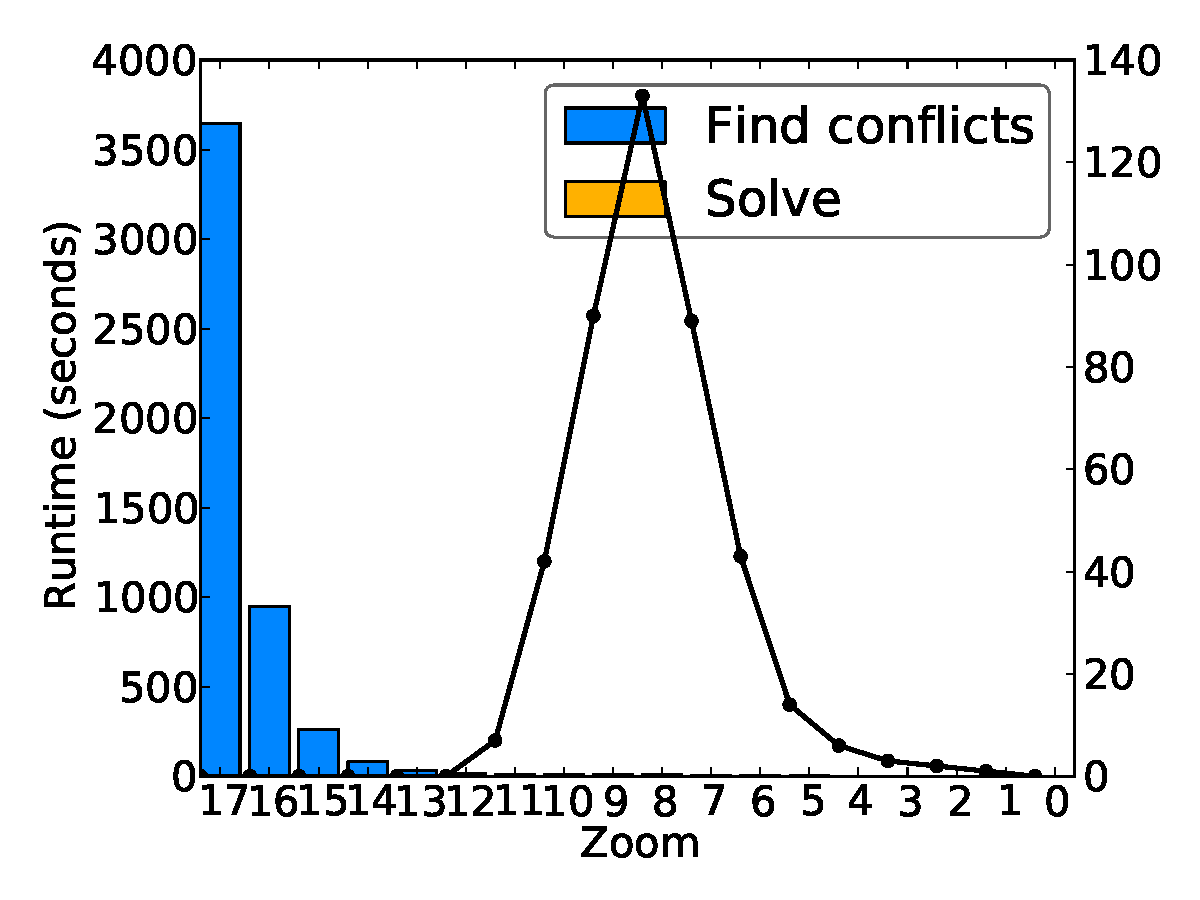
\includegraphics[width=0.9\linewidth]{figs-cvl/prelim_lin_30k_uswaterway_lp_A.pdf}}
    \centerline{(a) LPGA + Visibility}
  \end{minipage} \hfill
  \begin{minipage}{0.329\linewidth}
    \centerline{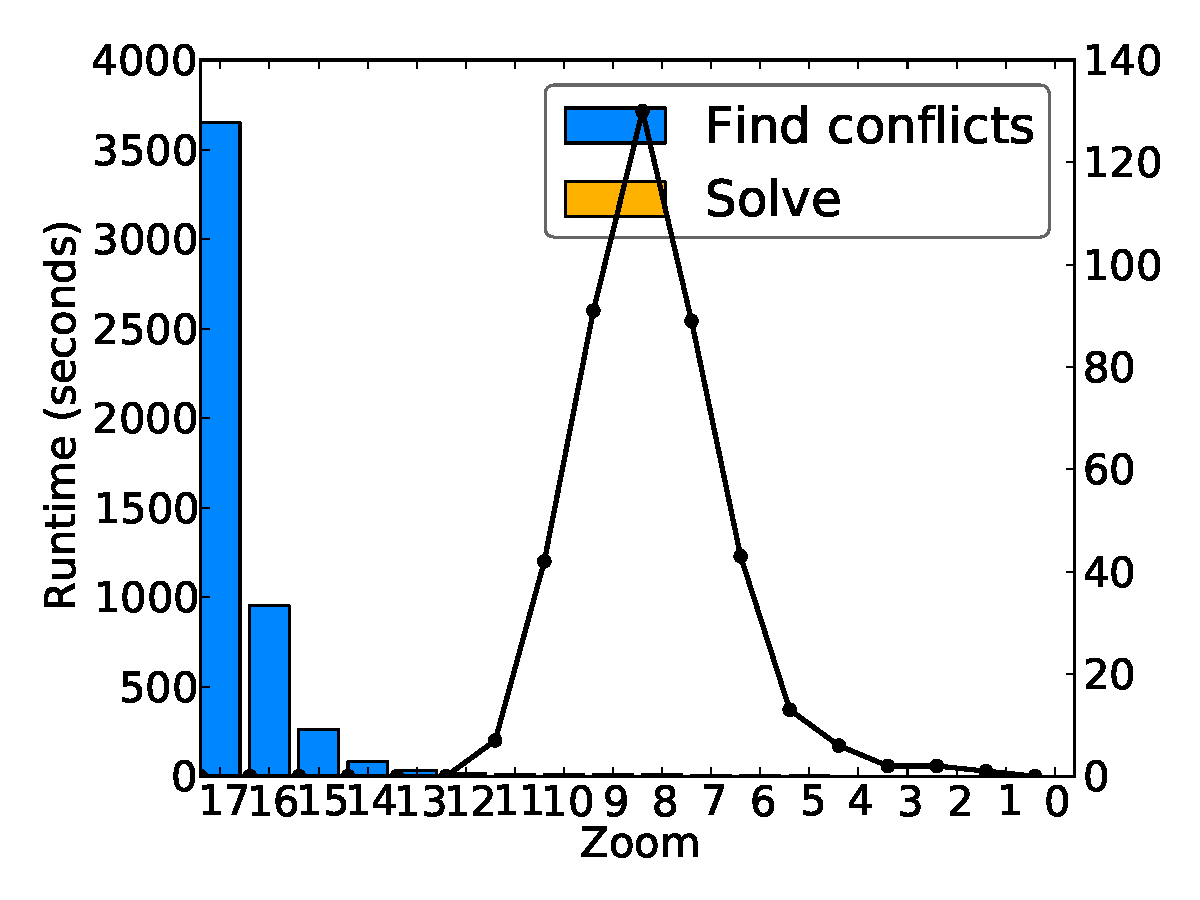
\includegraphics[width=0.9\linewidth]{figs-cvl/prelim_lin_30k_uswaterway_heuristic_A.pdf}}
    \centerline{(b) SGA + Visibility}
  \end{minipage} \hfill
  \begin{minipage}{0.329\linewidth}
    \centerline{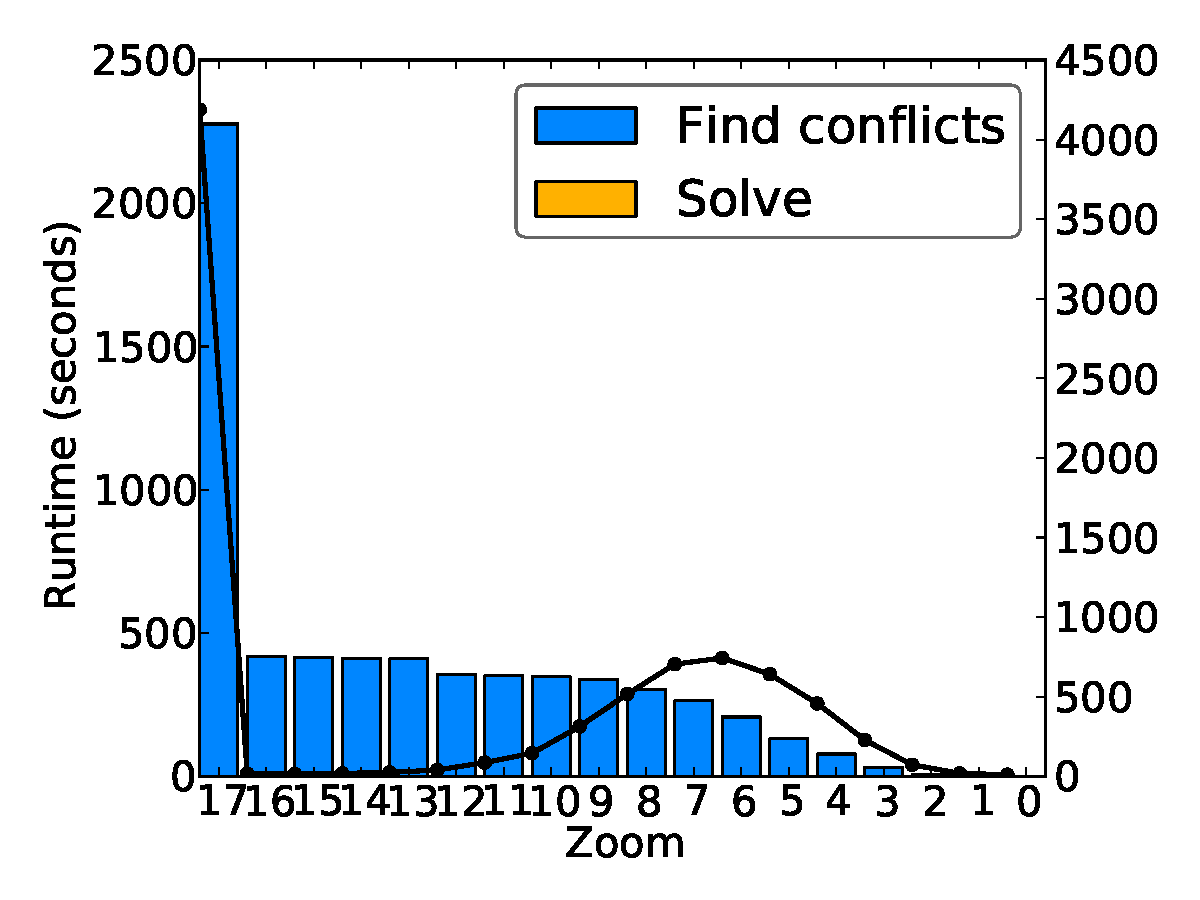
\includegraphics[width=0.9\linewidth]{figs-cvl/prelim_lin_30k_uswaterway_lp_B.pdf}}
    \centerline{(c) LPGA + Proximity}
  \end{minipage}
%  \vspace{-1ex}
  \caption{Performance breakdown by zoom level, Rivers dataset (4K records). The black line indicates number of conflicts} \label{fig:performance:complex}
%\vspace{-2ex}
\end{figure*}


\minisec{Performance breakdown}
In Figure~\ref{fig:performance:complex}, we show three performance breakdowns for the Rivers dataset. We make two observations. First, the running time is now completely dominated by finding conflicts. This is because the complexity of finding conflicts depends on the fidelity of the geometries that are compared. 
%For the proximity constraint, the complexity is proportional to the product of point counts for the two geometries compared in the distance test. For the visibility constraint, the complexity depends on the number of tiles occupied by each geometry, which depends on either the length or the area of the geometry. The solving time does not directly depend on the geometric properties, only on the number and structure of conflicts.
Parts (a)-(c) illustrate the effect in more detail, with Part (a) in particular showing the breakdown of a solution with an average optimality ratio of $1.0$. We see that for complex shape datasets, the running time is mostly dominated by the time spent finding conflicts. Since finding conflicts operates over the geometric properties of the data, it requires time proportional at least to the number of points that make up each complex shape. When solving conflicts, the running time is independent of geometric complexity. Interestingly, the time necessary to find conflicts is so high that it shadows the negative effect that a larger number of conflicts has on the conflict resolution time of LPGA (compare with Section~\ref{sec:exp:points}).

%This causes the running time to be dominated by finding conflicts for complex shape datasets. The LPGA solver is the exception when many conflicts are reported. A similar effect was seen for points, indicating that the LPGA solver does not scale well with the number of conflicts. %, which is confirmed in our scalability experiments.

\minisec{Scalability}
In Figure~\ref{fig:scalability}(b), we show scalability results for complex shape data. Here scalability depends more on the choice of constraint than on the choice of solver. The proximity constraint scales much worse than the visibility constraint with the number of objects. This is because the running time of the distance test used in the proximity constraint is proportional to the product of point counts in the two geometric shapes used in each comparison. In contrast, evaluating the visibility constraint depends on the number of tiles that each shape intersects, which depends more on the length or area of each shape. 

While constraints matter more to scalability for complex shapes than for point data, the SGA solver scales better than LPGA with number of objects, which was also the case for the point datasets examined in Section~\ref{sec:exp:points}.

\section{Related work}
\label{sec:related}

Cartographic generalization is a classic topic of investigation in the GIS community, and several models have been developed for generalization operations~\cite{harrie2007modelling}. While the problem has been considered by some as AI complete~\cite{frank1994multiscaletree}, recent work has focused on automatic map generalization based on optimization models or queries for filtering~\cite{sarma2012fusiontables,nutanong2012multiresolution}. This reduction in scope reflects the need of providing a wide variety of web-accessible maps summarizing ever increasing amounts of geospatial datasets. Our work provides support for the same trend.  

The optimization approach of Das Sarma et al.~\cite{sarma2012fusiontables} is the most related to our work. In contrast to our approach, however, Das Sarma et al. do not provide a flexible declarative interface for user-defined constraints, nor does their approach leverage SQL. 
%As a consequence, their approach is restricted to memory-resident datasets and pre-specified, not user-defined, constraints. 
In addition, it is hard to integrate their approach with existing geospatial data serving infrastructures, which are mostly based on standard spatial database technology.

User-defined constraints and declarative specifications have been shown to yield elegant solutions to a variety of problems in data management, including record deduplication~\cite{ArasuRS09:Dedupalog}, database testing~\cite{BinnigKL07:ReverseQP,Binnig:2007:SymbolicQP}, as well as cloud and networking resource optimization~\cite{Liu:2012:Cologne}. Our work brings these ideas to the context of map generalization and geospatial data, and as mentioned previously, is among the first frameworks to implement the vision of reverse data management~\cite{meliou2011reverse}. 

In-database processing has also been explored successfully in diverse contexts in the literature. Translation of high-level languages, such as XQuery or LINQ, to SQL lead to highly scalable and efficient implementations~\cite{pathfinder,ferry}. A number of recent approaches have targeted expressing complex statistical analytics in SQL~\cite{Hellerstein:2012:Madlib,Ordonez2007:StatisticsUDFs}. In contrast, we show how in-database processing can be used in the implementation of a declarative language for map generalization which includes solvers and constraints, leveraging the trend to incorporate whole programming language interpreters and support for spatial data structures in database engines~\cite{Blakeley2008:DotNET}.  

Our approach dovetails with a number of techniques from the literature, which hold potential to further extend or complement it. First, we observe that the running time of the LP-based greedy algorithm (LPGA) is generally high. We implemented this algorithm because it provides a theoretical bound on the solution quality. We plan to explore other algorithms for set multicover, such as the greedy algorithm described by Rajagopalan and Vazirani~\cite{rajagopalan1998primal}, to improve running time compared to the LP-based greedy algorithm, while achieving good quality. An interesting challenge is how to express such algorithms entirely in SQL.

Second, this work considers only selection of objects. An important extension is to allow other data reduction operations, such as geometric transformation and aggregation of objects. While we believe that CVL could be adapted to these additional requirements, this would imply modeling alternative semantics and procedures for satisfying constraints in our framework.

Third, we would like to experiment with geospatially-aware parallel processing infrastructures, such as Hadoop-GIS~\cite{Aji:2013:HadoopGIS}, for even further scalability in computing map generalizations. Finally, once a map generalization is complete, the resulting map must be served to end-users. This problem is orthogonal to our work, and classic linearization techniques can be applied~\cite{hilbert1891ueber}. All of these are interesting avenues for future work.

\section{Conclusion}

In this paper, we present a novel declarative approach to the data reduction problem in map generalization. 
%The proposed approach is complete in the sense that it integrates seamlessly with existing database and cartographic generalization technology. 
The proposed approach integrates seamlessly with existing database technology, and allows users to specify, using the proposed CVL language, and across all scales, what goals and constraints the generated map should fulfill --- leaving the detailed selection decisions to the system. The system leverages an algorithmic mapping which enables at the same time user-defined constraints and reuse of methods from the optimization literature. Our experiments show that the approach performs well for off-line processing and produces maps of high quality.

\section{Acknowledgements}
This project has been funded by Grontmij, the Danish Geodata Agency and the Ministry of Innovation in Denmark. We would like to thank employees and management at Grontmij and the Danish Geodata Agency for great discussions about the ideas presented in this work. We would also like to thank the anonymous reviewers for their insightful comments on our work. Finally, we would like to thank Amazon for providing an AWS in Education research grant award, which we used to implement our experimental setup.  

% !TEX root = ./thesis.tex
\chapter{Declarative Multi-scale Visualization of Large Graphs}

% Define clear usecase
% - Zoomable visualizations of large social networks

We want to:
\begin{itemize}
\item Model all data as graphs, because graphs are general (they subsume spatial, temporal and social data). 
\item Analyze graphs using zoomable graph visualizations
\item Share visualizations with the world
\item Support declarative languages for creating zoomable graph visualizations
\end{itemize}

We assume that there:

\begin{itemize}
\item Exists methods for translating any data into nodes and edges form; we will give examples
\item Exists methods for embedding nodes and edges in the plane, i.e. computing two-dimensional coordinates for nodes and edges
\end{itemize}

For this to work, we must:
\begin{itemize}
\item Define a notion of \emph{resolution} or \emph{scale} for graphs; it is sufficient to define a unit for the two-dimensional coordinate system, e.g. meters
\item Define a query model for graph views, e.g. the pyramid model because it is scalable
\item Define metrics for evaluating graph views, e.g. information density metrics (see Woodruff et al.~\cite{woodruff1998constant})
\item Define valid transformation functions for turning one graph into another graph

\item Formulate constraints that can be evaluated over graph views
\item Define a distance function 
\item Define an equivalence relation between graph views at different scales, i.e. what are the constraints that must hold when transforming graphs between scales

\item Define metrics for evaluating scale-based views for graphs, e.g. density metric


We need to guide the abstraction process, i.e. objective functions. 

We want the multi-scale data abstraction of graphs to be user-programmable, to support data enthusiasts and professional analysis. We need scalable algorithms and systems that implement the whole deal.

\end{itemize}

% Motivation

\section{Introduction}

\section{Multi-scale Graph Abstraction}
We want to compute a multi-scale data abstraction for a graph. at a set of discrete scales. For this we need to: Model data (i.e. spatial, temporal, social data) as graphs. Define a scale-based view of graphs (projection of graph into metric space, representation of metric space in pixel space). Define equivalence classes for graphs (subject to constraints)
\subsection{Modeling Data Domains}
% how can we model different domains as graphs
% - spatial
% - temporal
% - 
\subsection{Scale-based View Model}

\subsection{Data Abstraction Operators}
\subsection{Equivalent Graphs}
\paragraph{Graph Minor}
\paragraph{Constraints}


\section{Modeling}
\subsection{Data Model}
\subsection{Query Model}
\subsection{Graph Projection}
\subsection{Scale-based Equivalence}

\section{Related Work}

\section{Conclusion}
\part{Scalable Geospatial Data Serving}
% !TEX root = ./thesis.tex
\chapter{Overview of State-of-the Art Geospatial Data Serving}

\section{Spatial Indexing}
% vector tiles, r-trees, linearization

% !TEX root = ./thesis.tex
\chapter{TileHeat: A Framework for Tile Selection}
% abstract
Public geospatial services are now commonly available on the Web. These services often render maps to users by dividing the maps into tiles. Given that geospatial services experience significant user load, it is desirable to pre-compute tiles at a time of low load in order to increase overall performance. Based on our analysis of the request log of a public geospatial service provider, we observe that times of low load occur with a periodic pattern. In addition, our analysis shows that tile access patterns exhibit strong spatial skew.

Based on these observations, we propose an adaptive strategy restricting the set of tiles that are pre-computed to fit the low load time window. Ideally, the restricted tile set should deliver performance comparable to the full tile set. To achieve this result, tiles should be selected based on their expected popularity. Our key observation is that the popularity of a tile can be estimated by analyzing the tiles that users have previously requested. Our adaptive strategy constructs heatmaps of previous requests and uses this information to decide which tiles to pre-compute. We examine two alternative heuristics, one of which exploits that nearby tiles have a high likelihood of having similar popularity. We evaluate our methods against a real production workload, and observe that the latter heuristic achieves a 25\% increase in the hit ratio compared to current methods, without pre-computing a larger set of tiles.

\section{Introduction}

% Situation
Today geospatial web services are widely deployed on the web. A significant subset of these services can be queried using bounding box requests to retrieve geospatial data, either in raster or vector form, within a region. The classic example of such a service is Web Map Service (WMS). In WMS, results are typically computed on-the-fly by pulling data from a geospatial database. This strategy has the advantage that results are always up-to-date and it thus offers a great degree of flexibility and accuracy to clients of the service. At a high level, we can think of the service as applying a \emph{rendering function} to a set of matched base data to produce, e.g., a map image.

% Problem
Services that apply rendering functions in response to bounding box requests are often CPU- and I/O-intensive, with relatively high latency as a consequence. This is a problem because geospatial services are typically used interactively, and latency in excess of a few hundreds of milliseconds becomes noticeable. Even if the computation is not that expensive, the infrastructure available might not scale to many simultaneous users, if data is to be computed on demand. We know from our studies of government production services that may use as much as 30 seconds to compute a 256 x 256 pixel map image, which severely lowers the value of the service in an interactive scenario. On the other side, limiting the use of GIS to working with results that can be computed fast, does not generally seem like a good idea. While the issue of high latency can to a certain degree be dealt with by scaling up or out, such solutions do not come without a cost, e.g. increased power consumption and hardware costs. Instead of simply adding more resources, better algorithms can be developed to deal with high latency.

% State of the art
Real-world workloads contain significant amounts of repeated requests and often a strong skew in what is requested~\cite{fisher07,talagala00}. This offers an opportunity to replay the results of previous computations by placing geospatial results in a cache. A common approach to representing a set of geospatial results at multiple resolutions is to use a tiling scheme that divides a geographical data set into a hierarchical and finite set of \emph{tiles}~\cite{decola93}. Unfortunately, the drawback of this approach is that the set of tiles is potentially very large~\cite{garcia11}, as the number of tiles is exponential in the number of supported resolutions. It is common to fix the number of resolutions when dealing with tiles, and thus we assume a fixed set of resolutions. Even then, the sheer number of tiles makes computing and storing all of them difficult to manage.

Two primary approaches have been suggested for dealing with the delivery of tiles to clients: \emph{online} and \emph{off-line}. The online approach attempts to mask the latency of computing tiles on-demand for a single user, by prefetching tiles based on predictions of future accesses given the user's current viewstate~\cite{KKK01:Prefetching,KKK01:Prefetching2,LKK+02:Prefetching}. The off-line approach is to materialize a large but polynomial number of tiles in advance that is expected to cover to the majority of user request in the near future. It is assumed that serving the materialized tiles from a cache will be less CPU- and I/O-intensive than computing them on demand. The main problem then becomes selecting a good set of tiles. 

A drawback to the online approach is that although pre-fetching theoretically masks latency for a single user, it does not by itself decrease global concurrency, as tiles are still computed on demand. We speculate that this approach could even increase the average latency if view states are mispredicted. A drawback with materializing a set of tiles offline is that the tiles might not be up-to-date by the time they are requested, but this can be solved by invalidating the stale tiles. We will focus on the latter off-line approach in our work.

The off-line approach takes a global view of the problem, and aims at predicting a ``good'' set of tiles, i.e., a set containing tiles that are likely to be requested by many users in the near future. We argue that these tiles should be materialized during a window of low load. This strategy avoids impacting latency negatively in the high load period, but holds the potential to reduce average latency because of pre-computation.

% which in turn increases the average global latency, in order to decrease the latency for a particular user. 
Methods in the literature use rule-based algorithms to select which tiles should be materialized ahead of time~\cite{quinn10}. The rules are based on \emph{a priori} knowledge of user behavior, so a drawback of these methods is that the rules do not adapt to changes in user behavior over time. In addition, rule-based methods are hard to adapt to shorter time windows of low load. As they offer only limited insight over which tiles are the most relevant among the tiles selected by the rules, it is hard to choose a good subset of tiles to be materialized under a time constraint.  
% MVS: are there other rule-based approaches that we can cite? Does anybody cite Quinn and Gahegan?

In this paper, we present an adaptive tile selection method, \emph{TileHeat}, which suffers significantly less from these drawbacks. TileHeat is based on  \emph{a posteriori} knowledge of user behavior gathered from historical usage of the geospatial web service. We investigate algorithms that predict the set of tiles that will be requested in time period $t + 1$, and that are trained using a log of requests for periods $t-n, t -n + 1, \ldots, t$. Our algorithms construct a set of $n$ spatial heatmaps of requests, one for each time period, and uses these to predict future requests. To avoid over-fitting the model to the training data, we use both exponential smoothing and heat dissipation on the constructed heatmaps. The output of our algorithms is a ranking of tiles based on predicted likelihood of access for the next time period. As such, the number of tiles to be pre-computed can be chosen according to the available time window of low load.	

\minisec{Outline and Contributions}
Our paper starts with a discussion of existing methodologies for tile caching (Section~\ref{sec:tile:caching}). Then the main \emph{contributions} of the paper follow:
%
\begin{itemize}

\item We analyze a sample from the production log of The Digital Map Supply, a production geospatial web service maintained by the National Survey and Cadastre (KMS) in Denmark. In Section~\ref{sec:analysis}, we present our key observations of the workload, e.g. that the load curve follows a pattern with high load in the middle of the day, and low load in the rest of the day, and that the spatial distribution of requests is very stable over time.

\item We present the general framework of TileHeat, and propose a set of algorithms for ranking tiles. The algorithms exploit the properties we have discovered in the analysis, namely by tracking and predicting the spatial distribution of requests using heatmaps (Section~\ref{sec:algorithms}).

\item We present an experimental evaluation of the effectiveness of TileHeat. We observe an improvement of $25\%$ over the existing method used in the production system of KMS  for a set of tiles that can be materialized during an observed time window of low load (Section~\ref{sec:experiments}).

\end{itemize}
%
We end the paper by reviewing additional related work (Section~\ref{sec:related}). 

\section{Background}
\label{sec:tile:caching}

A \emph{tile cache} is a widely used method for dealing with the bad performance of services that render results from base data on-the-fly, such as WMS and similar services. In the following, we discuss the main concepts (Sections~\ref{sec:tile:pyramid} to~\ref{sec:heatmap:model}) and existing methods (Section~\ref{sec:existing:methods}) in tile caching.

\subsection{The Tile Pyramid}
\label{sec:tile:pyramid}

Tile caches are based on a model called a \emph{tile pyramid}, which subdivides a geographical region into a finite number of subregions using a set of $l$ grids~\cite{decola93}. In Figure~\ref{fig:tilepyramid}, a tile pyramid with three levels is shown. The cells of the grids are called \emph{tiles}, and tiles are indexed by a triple $(i,j,z)$. In this triple $z$ identifies a grid, while $i$ and $j$ represent the row and column in the grid where the tile is located. Each grid is associated with a data set at a particular resolution in meters per pixel. Tiles thus correspond to data at a given resolution, and within a bounding box.

\begin{figure}
\centering
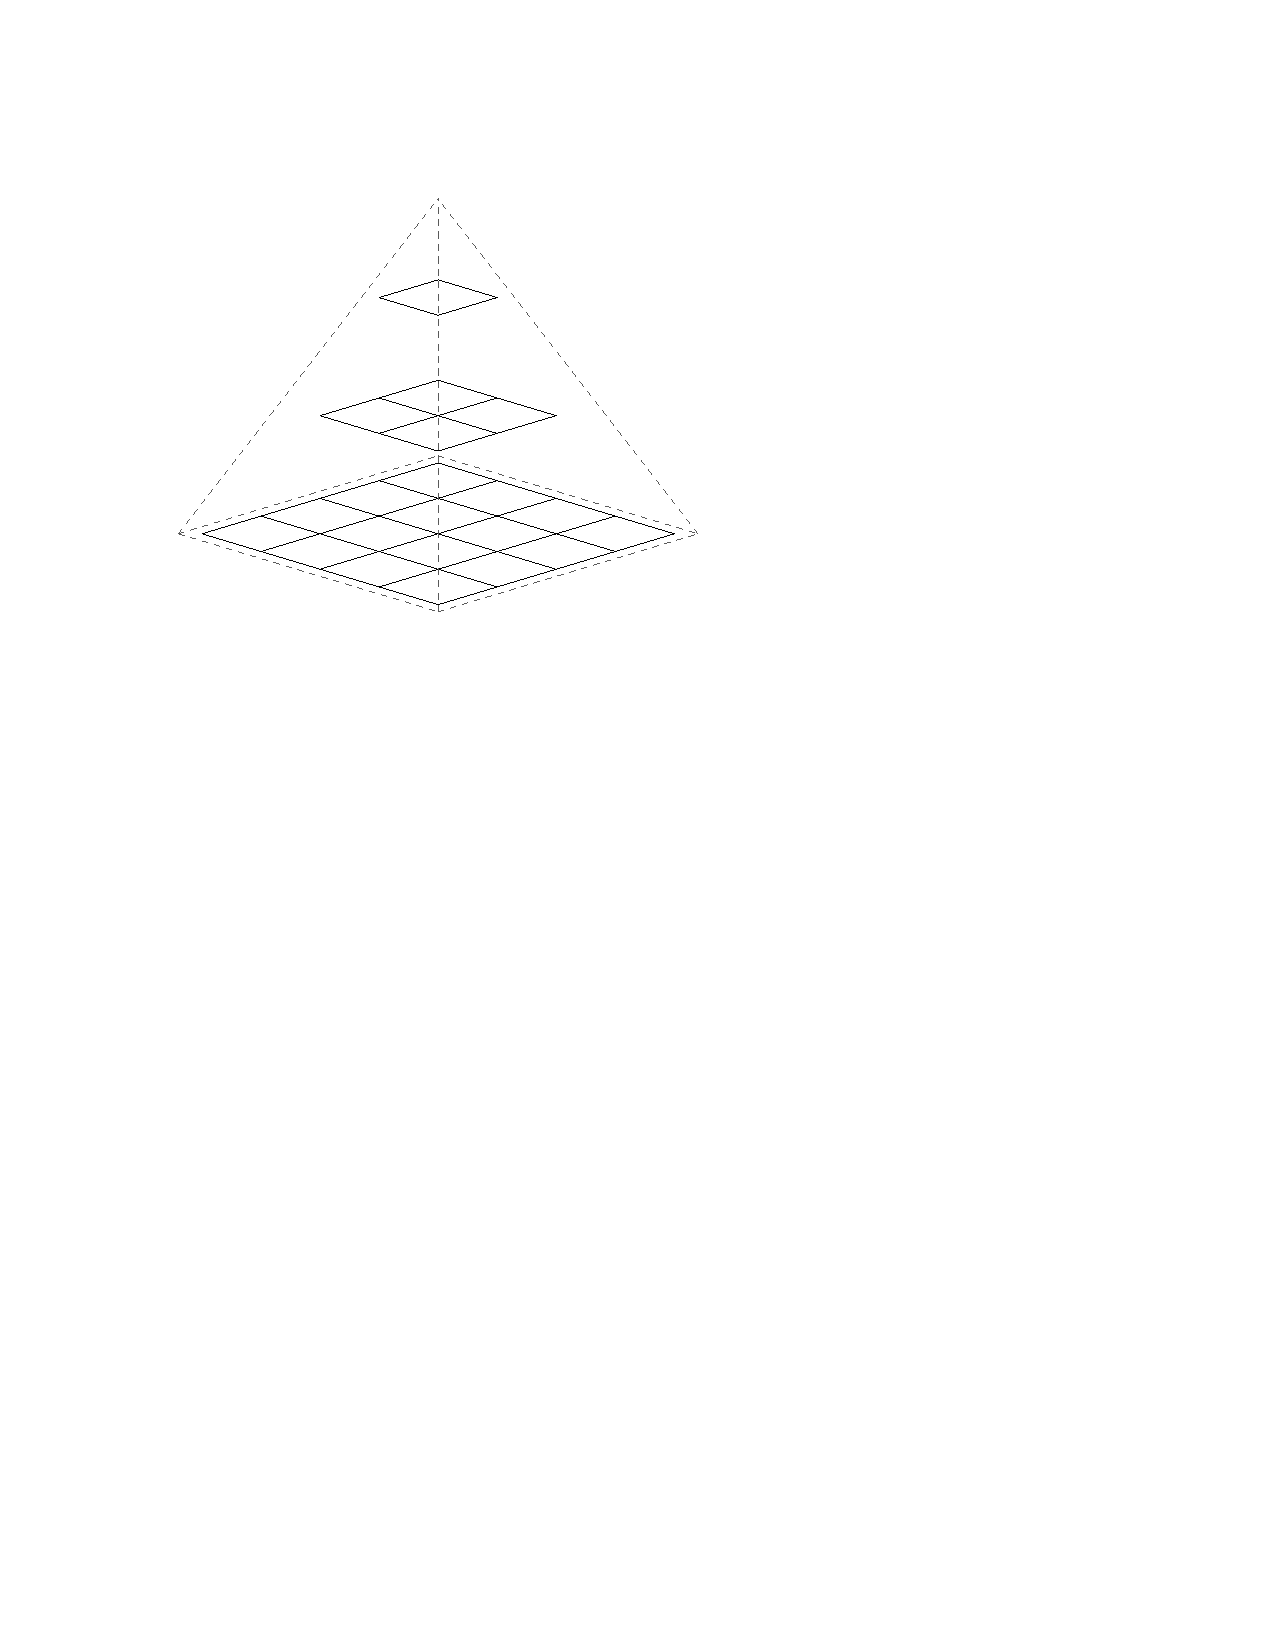
\includegraphics[scale=0.8]{figs-tileheat/tilepyramid}
\caption{Tile pyramid with three levels $z=\{1, 2, 3\}$ shown. Level $z=1$ has dimensions $(1,1)$. Figure is reproduced from \cite{quinn10}}
\label{fig:tilepyramid}
\end{figure}

When a tile cache is initialized, all tiles point to $null$. A tile is materialized by making it point to geographical data stored on disk. The geographical data is rendered from a set of base objects, and if the base objects are updated the tile becomes \emph{stale}. Stale tiles are removed to avoid serving stale data to clients.

One shortcoming of tile caches is that the number of tiles is exponential in $l$, with grid $i+1$ containing four times as many tiles as grid $i$. This means that a tile cache consumes $O(4^l)$ in storage, and $O(4^l)$ time is required to materialize all tiles. A pyramid of $l=20$ levels requires several petabytes of storage \cite{garcia11}. The throughput of computing tiles has been reported by KMS to be around $58$ tiles per second on their infrastructure \cite{lindegaard12}. At this rate of computing tiles, it would take approximately $200$ years to compute the $3.7 \times 10^{11}$ tiles needed~\cite{garcia11}.

\subsection{Processing user requests}
\label{sec:processing:user:requests}
We abstract user requests to a geospatial web service by two functions: \texttt{GET} and \texttt{PUT}. \texttt{GET} retrieves a tile from a web service, while \texttt{PUT} updates the base data from which tiles are computed. Pseudocode for processing \texttt{GET} and \texttt{PUT} requests are given in Figure \ref{fig:pseudocode}.

\begin{figure}[h]
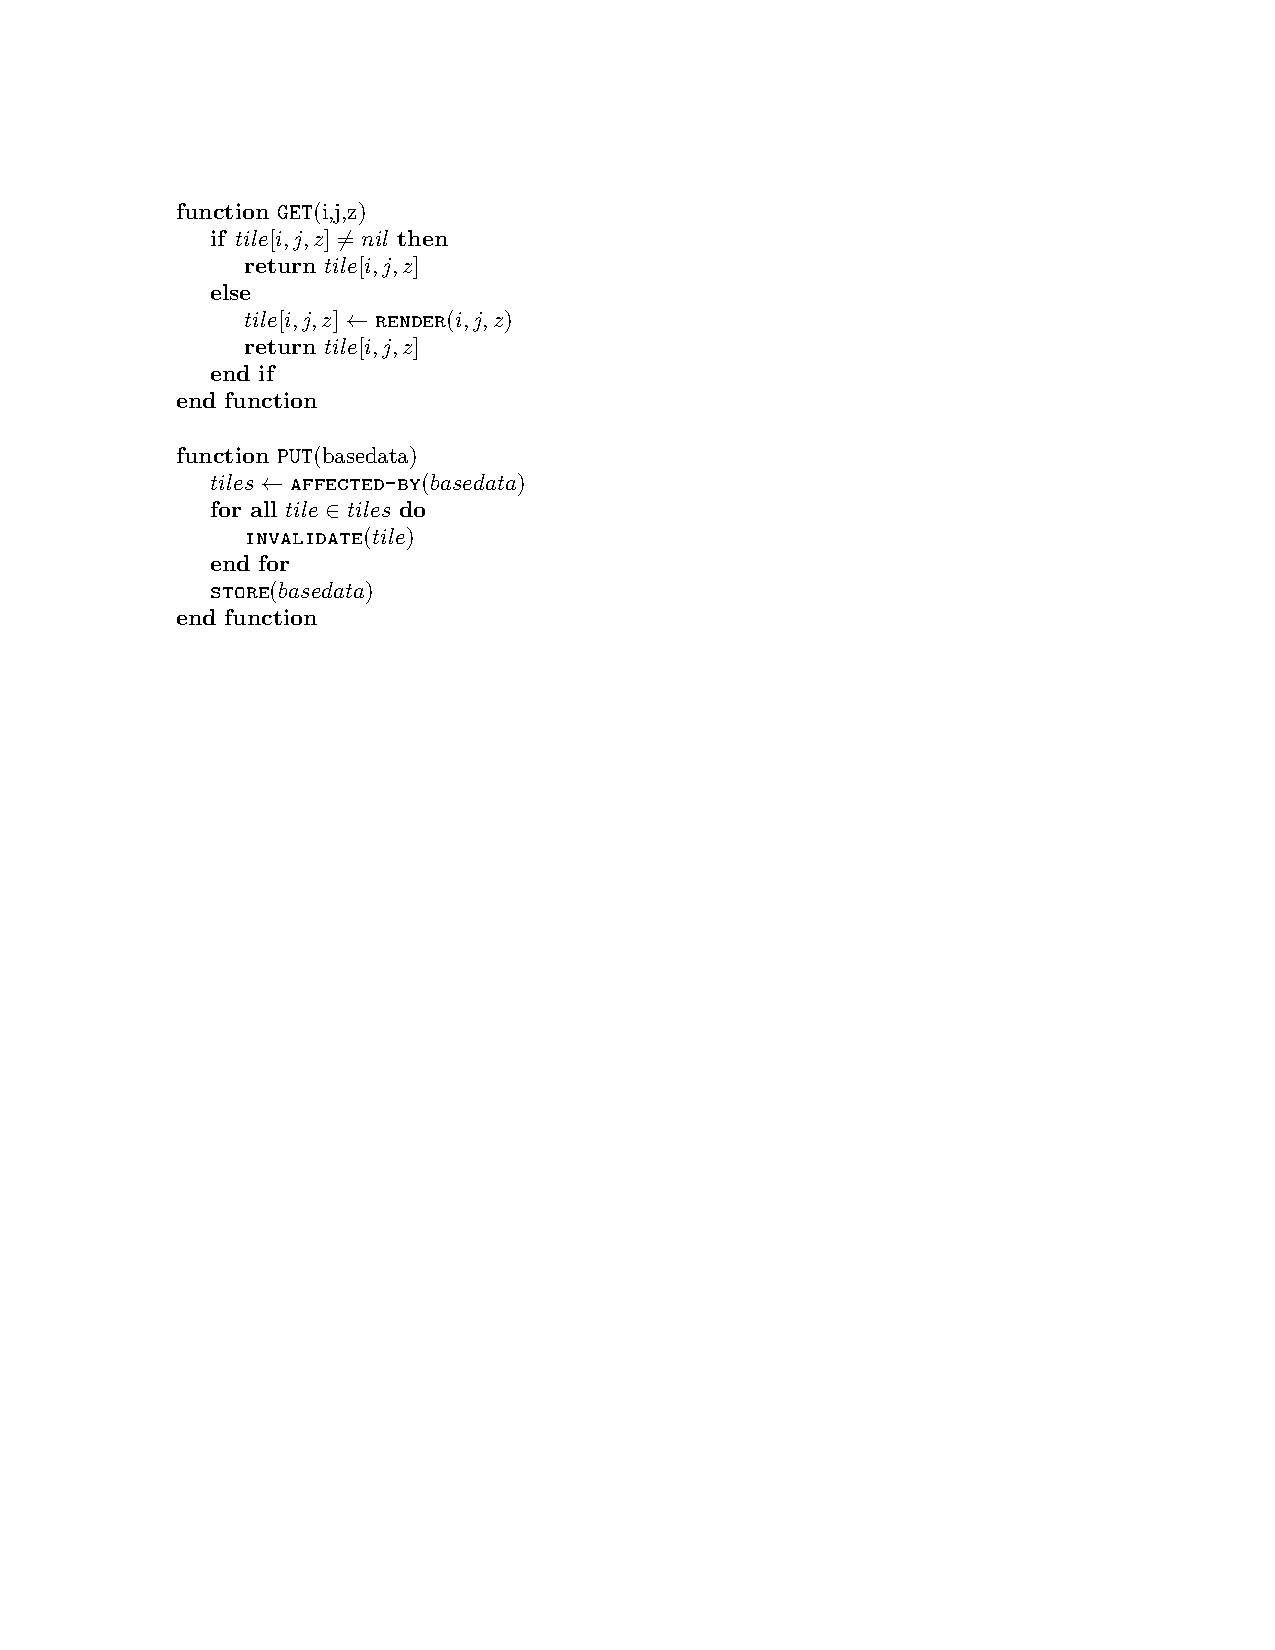
\includegraphics[scale=0.9]{figs-tileheat/pseudocode}
\caption{Processing a \texttt{GET} request: If the tile is materialized, it is returned. Otherwise it is rendered, stored and returned. Processing a \texttt{PUT} request: When base data is updated, the set of tiles that is affected by the change needs to be invalidated.}
\label{fig:pseudocode}
\end{figure}

An invariant maintained by the above functions is that stale tiles are never returned to the user. However, one implementation difficulty typically encountered in practice is that the method for determining the set of tiles that are affected by an update to the base data is not entirely accurate, i.e., a conservative estimate is used in function \texttt{AFFECTED-BY}. This means that sometimes tiles are unnecessarily discarded.

A bounding box request, such as a WMS request, can easily be modeled as a set of \texttt{GET} requests by computing the set of tiles that are intersected inside the \emph{nearest} grid of the tile pyramid. By nearest, we mean the grid that contains tiles with a resolution that best matches the resolution of the bounding box request. Note that these multiple \texttt{GET} requests must be processed against a consistent snapshot. 
%Description of the appropriate implementation details are however beyond the scope of this paper. 

\subsection{The Heatmap model}
\label{sec:heatmap:model}
Given a set of \texttt{GET} requests, we can generate a heatmap of the requests \cite{fisher07}. A heatmap quantifies the number of requests $h_{i,j,z}^t$ that a tile with index $(i,j,z)$ has received in time period $t$. We consider multi-scale heatmaps, which are associated with a tile pyramid. In this work, we only use heatmaps to measure the number of \texttt{GET} requests per tile, but other request types could also be tracked with heatmaps. For example, we could generate heatmaps of \texttt{INVALIDATE} requests, but this is outside the scope of our work.

\subsection{Existing Methods}
\label{sec:existing:methods}
This section covers existing methods for computing and storing a set of tiles for a tile cache.

\minisec{Parallel processing}
Clearly, we need techniques to speed the computation of a tile cache up, given that the number of tiles in a tile pyramid is huge. Using a parallel programming model such as MapReduce \cite{dean04} could reduce computation time of a tile cache by a large factor, but it would require a significant number of machines. In other words, parallelism improves time-to-solution, but does not reduce the amount of resources necessary for the computation. For organizations such as KMS, this high resource cost renders the use of brute-force parallelism unfeasible. A solution is called for to reduce the number of tiles that needs to be computed --- which could then be orthogonally combined with parallelism if available.

\minisec{Detecting duplicates}
A method that reduces storage requirements is to exploit that many tiles are identical, e.g., blue ocean tiles~\cite{mbtile12}. Unfortunately, this solution does not necessarily reduce computation time, given that tiles often must be computed in order to check that they are duplicates. Heuristics have been suggested to predict these duplicated tiles without full computation, but it is unfortunately not easy to decide with absolute certainty~\cite{mbtile12}. We do not know of any published methods that accurately and efficiently predict whether two tiles are the same in the general case without actually computing them, because arbitrary rendering functions are employed.

\minisec{Tile Caching based on Geometries}
A number of authors have suggested methods for predicting the popularity of tiles. Quinn and Gahegan~\cite{quinn10} suggest using certain classes of base objects, like roads and coastlines, as predictors of where people will look at a map. Tiles that are at most 3 miles away from the selected predictors are cached. Conceptually, this approach is based on a model of rational user behavior with fixed rules, and historical workloads are used only to validate the model.

\minisec{GEOM}
KMS currently uses a simplified version of the approach above, which we term \emph{GEOM}. A set of polygons that roughly cover the land areas of Denmark are used to identify the areas that should be fully materialized at all levels of the tile pyramid (levels 1 to 12). Areas outside of these polygons are only materialized at the top-most levels of the tile pyramid (levels 1 to 6)~\cite{lindegaard12}. The resulting partial cache is manageable in size, as roughly $10\%$ of the tile pyramid is materialized. However, the computation time is reported to be between $1.5$ and $2$ days. Tiles are generated by going row-by-row down the levels of the tile pyramid. This is significantly better than random selection, as the highly popular tiles near the top of the pyramid are generated early.

\section{Analysis}
\label{sec:analysis}

In this section, we analyze the request log of a production geospatial web service within KMS, and observe a number of interesting patterns.
The service we examine is the most popular web service of the The Digital Map Supply, a WMS that receives around 800,000 requests per day, and delivers a general purpose background map of Denmark. We report on both temporal (Section~\ref{sec:temporal:characteristics}) and spatial (Section~\ref{sec:spatial:characteristics}) characteristics of the workload.

\subsection{Temporal characteristics of workload}
\label{sec:temporal:characteristics}

\begin{figure}
\centering
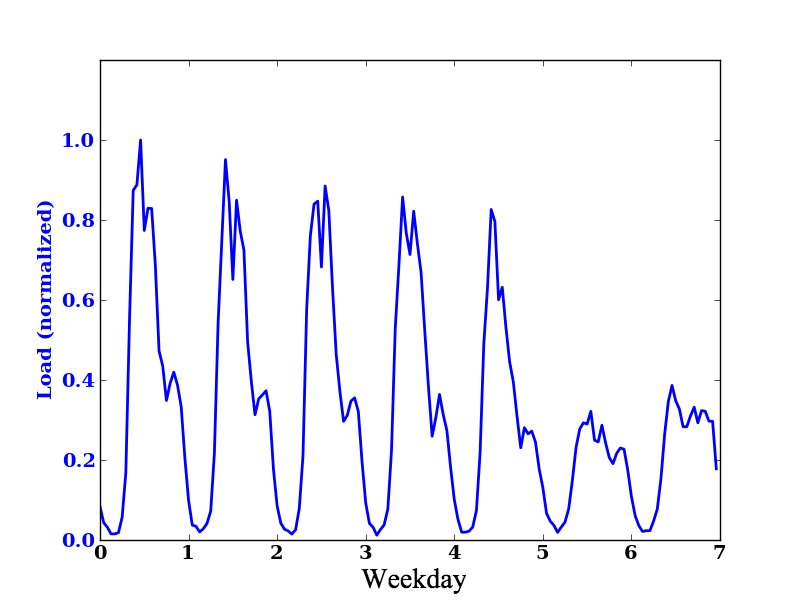
\includegraphics[scale=0.4]{figs-tileheat/average_load_week.png}
\caption{Average load per hour for each day of the week.}
\label{fig:weekload}
\end{figure}

Using a random sample of 90,000 WMS requests from the log, we analyze the workload over time. We have found the following when examining requests processed per second:

\begin{itemize}
\item The load is consistently higher during the middle part of the day, than during other parts of the day.
\item The 24-hour load curves for any two weekdays are very similar.
\item The 24-hour load curves for Saturdays and Sundays are very similar.
\item In general, the load is much higher during weekdays, compared to weekends.
\end{itemize}

These patterns are shown in Figure~\ref{fig:weekload}, where we display the average 24-hour load curve for each day of the week. The curve is generated as an average of all weeks in the log.

\begin{figure}
\centering
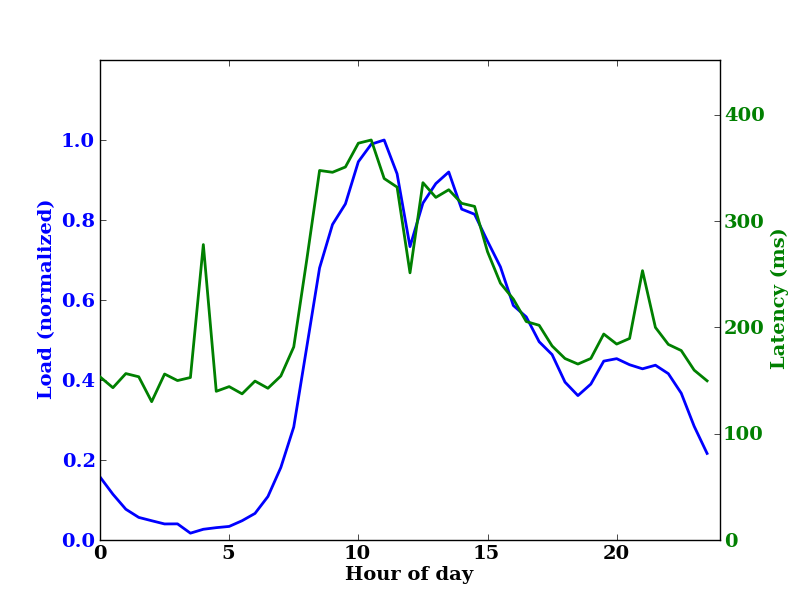
\includegraphics[scale=0.4]{figs-tileheat/correlation.png}
\caption{The correlation between average load (blue) and average latency (green) for 24-hour period.}
\label{fig:correlation}
\end{figure}

We have also looked at the effect of load on latency. In Figure~\ref{fig:correlation}, we plot, side-by-side, the average load and latency curves for a 24-hour period. We observe the following:

\begin{itemize}
\item Load and latency are highly correlated, especially during the periods of high load.
\item The latency effectively doubles when the load is high.
\item Given that weekdays have higher load than weekends, the degradation of latency is most severe in the middle of the day, on weekdays.
\end{itemize}

Our hypothesis is that the increase in latency is caused by increased concurrency and queueing in the system. We have also tested the stability of the load pattern over time by plotting the load for each day over a longer period within the last quarter of 2011. The load patterns can be seen in Figure~\ref{fig:anomaly}. We observe that in general the load curve is very consistent from one weekday to the next, and one week to the next, but anomalies do occur. During week 49 of the last quarter of 2011, the number of requests suddenly doubles. While it is not easy to know what caused such a load spike, it is interesting to ask whether the spike affects the spatial distribution of requests. We examine this question in Section~\ref{sec:spatial:characteristics}.

\begin{figure}
\centering
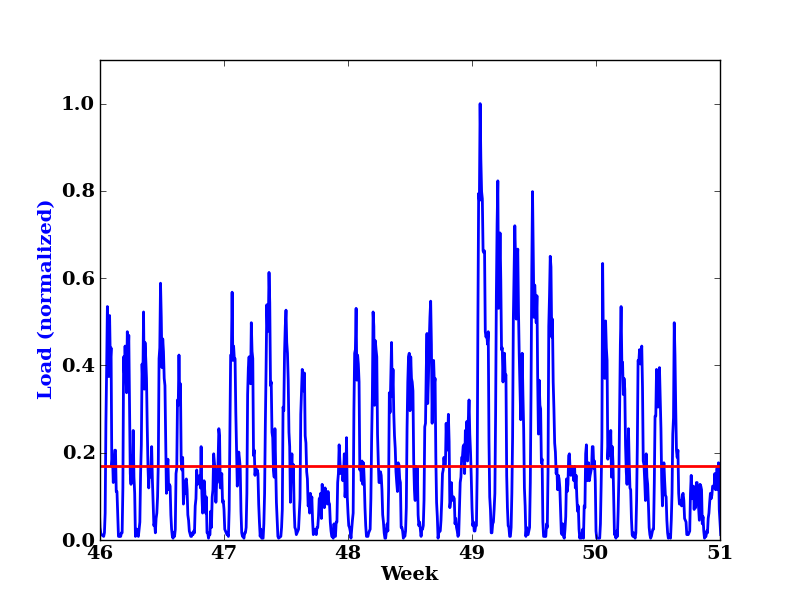
\includegraphics[scale=0.4]{figs-tileheat/anomaly.png}
\caption{Generally stable load, with an anomaly in week 49. The load almost doubles on the first day of week 49. The red line is the average load.}
\label{fig:anomaly}
\end{figure}

\subsection{Spatial characteristics of workload}
\label{sec:spatial:characteristics}
Using heatmaps we have investigated the spatial distribution of requests. We have selected a large number of weekdays, and extracted a full log for these days. The number of log records is significant, with more than 800,000 requests received per day. In Figure \ref{fig:heatmaps}, we show heatmaps for four of these days. We observe that the spatial distribution of requests is quite similar across days. We observe a similar pattern on other days from the log that we have examined.

Given the anomaly in requests per second that we noted in Figure~\ref{fig:anomaly}, we wanted to investigate if the spatial distribution of requests was different for days of increased load compared to normal days. The lower right part of Figure~\ref{fig:heatmaps} shows a heatmap for the day with unusually high load. The spatial distribution is slightly different compared to the other three heatmaps, but still very similar. The data indicates that the spatial distribution of requests is similar for weekdays, and largely independent of fluctuations in load. Using the notation we defined for heatmaps this means that

\[
h_{i,j,z}^t \approx h_{i,j,z}^{t+1}
\]

\begin{figure}
\centering
\begin{tabular}{|c|c|}
\hline
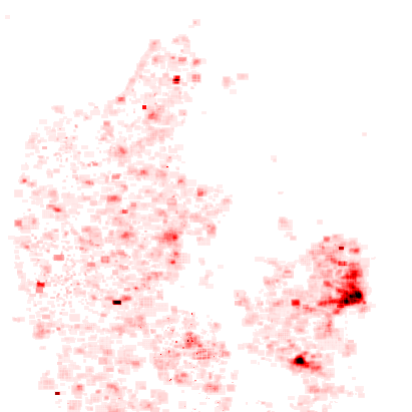
\includegraphics[scale=0.22]{figs-tileheat/heatmap-e_1.png} & 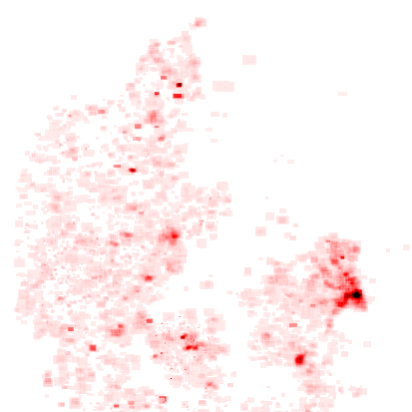
\includegraphics[scale=0.22]{figs-tileheat/heatmap-e_2.png} \\
\hline
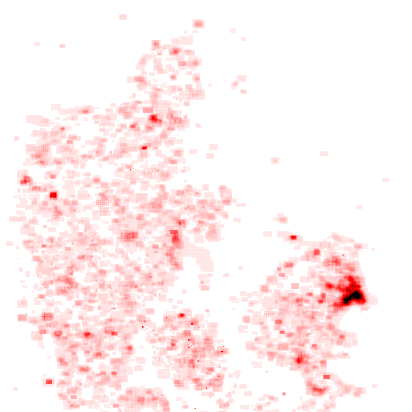
\includegraphics[scale=0.22]{figs-tileheat/heatmap-e_3.png} & 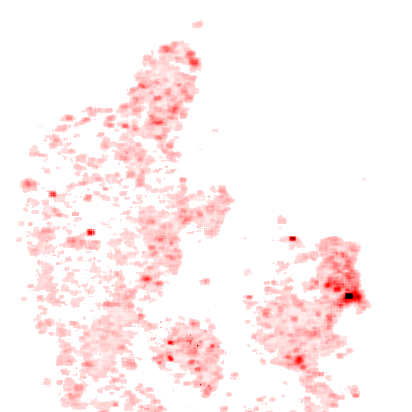
\includegraphics[scale=0.22]{figs-tileheat/heatmap-e_4.png} \\
\hline
\end{tabular}
\caption{Heatmap of spatial distribution of requests for four consecutive days (resolution $\mathbf{3.2}$ meter/pixel). The spatial distribution is similar but not equal. The day in the lower right corner is the day with very high load identified in Figure \ref{fig:anomaly}.}
\label{fig:heatmaps}
\end{figure}

%In Figure~\ref{fig:skew}, we show the cumulative distribution function of tile access frequencies, which has been computed from the heatmaps. 
We observe that the frequency of tile access is highly skewed; other studies have concluded the same, namely that the spatial distribution of \texttt{GET} requests follows a power law \cite{fisher07,talagala00}. We also observe that the skew increases with resolution, i.e., with  levels of the tile pyramid that contain more tiles. 

In general, this means that the set of tiles needed for a tile cache with a high hit ratio is smaller than one might expect. The main goal of our work and the algorithms we have developed is to explore how small such a cache can be, while still delivering high hit ratios on user requests.

\section{TileHeat framework}
\label{sec:algorithms}

In this section, we present the TileHeat framework for selecting and caching tiles. We begin with an overview of the framework and the context it is used in (Sections~\ref{sec:tileheat:overview} and~\ref{sec:tileheat:tasks}), followed by two different algorithms for tile ranking (Sections~\ref{sec:heat:hw} and~\ref{sec:heat:d}).   

\vspace{4ex}

\subsection{Overview}
\label{sec:tileheat:overview}
Based on our observations of the workload in Section \ref{sec:analysis}, we have designed the TileHeat framework for a repeated cycle of time periods containing a high- and low-load window. This basic cycle is outlined in Figure~\ref{fig:high:low}.

The life cycle of a system that uses TileHeat to manage tiles is as follows: We organize processing in TileHeat into a sequence of \emph{time periods}. Each time period is composed of two \emph{time windows}: the high-load window and the low-load window. Throughout both windows, the geospatial web service is available for clients and therefore must carry out normal processing of user requests, i.e., \texttt{GET} and \texttt{PUT}. During the low load window, however, we can additionally \emph{select and pre-compute tiles} that we expect to be accessed during the next time window, based on access patterns observed for previous time periods. In the following, we describe how we carry out the selection and pre-computation of tiles.

\begin{figure}
\centering
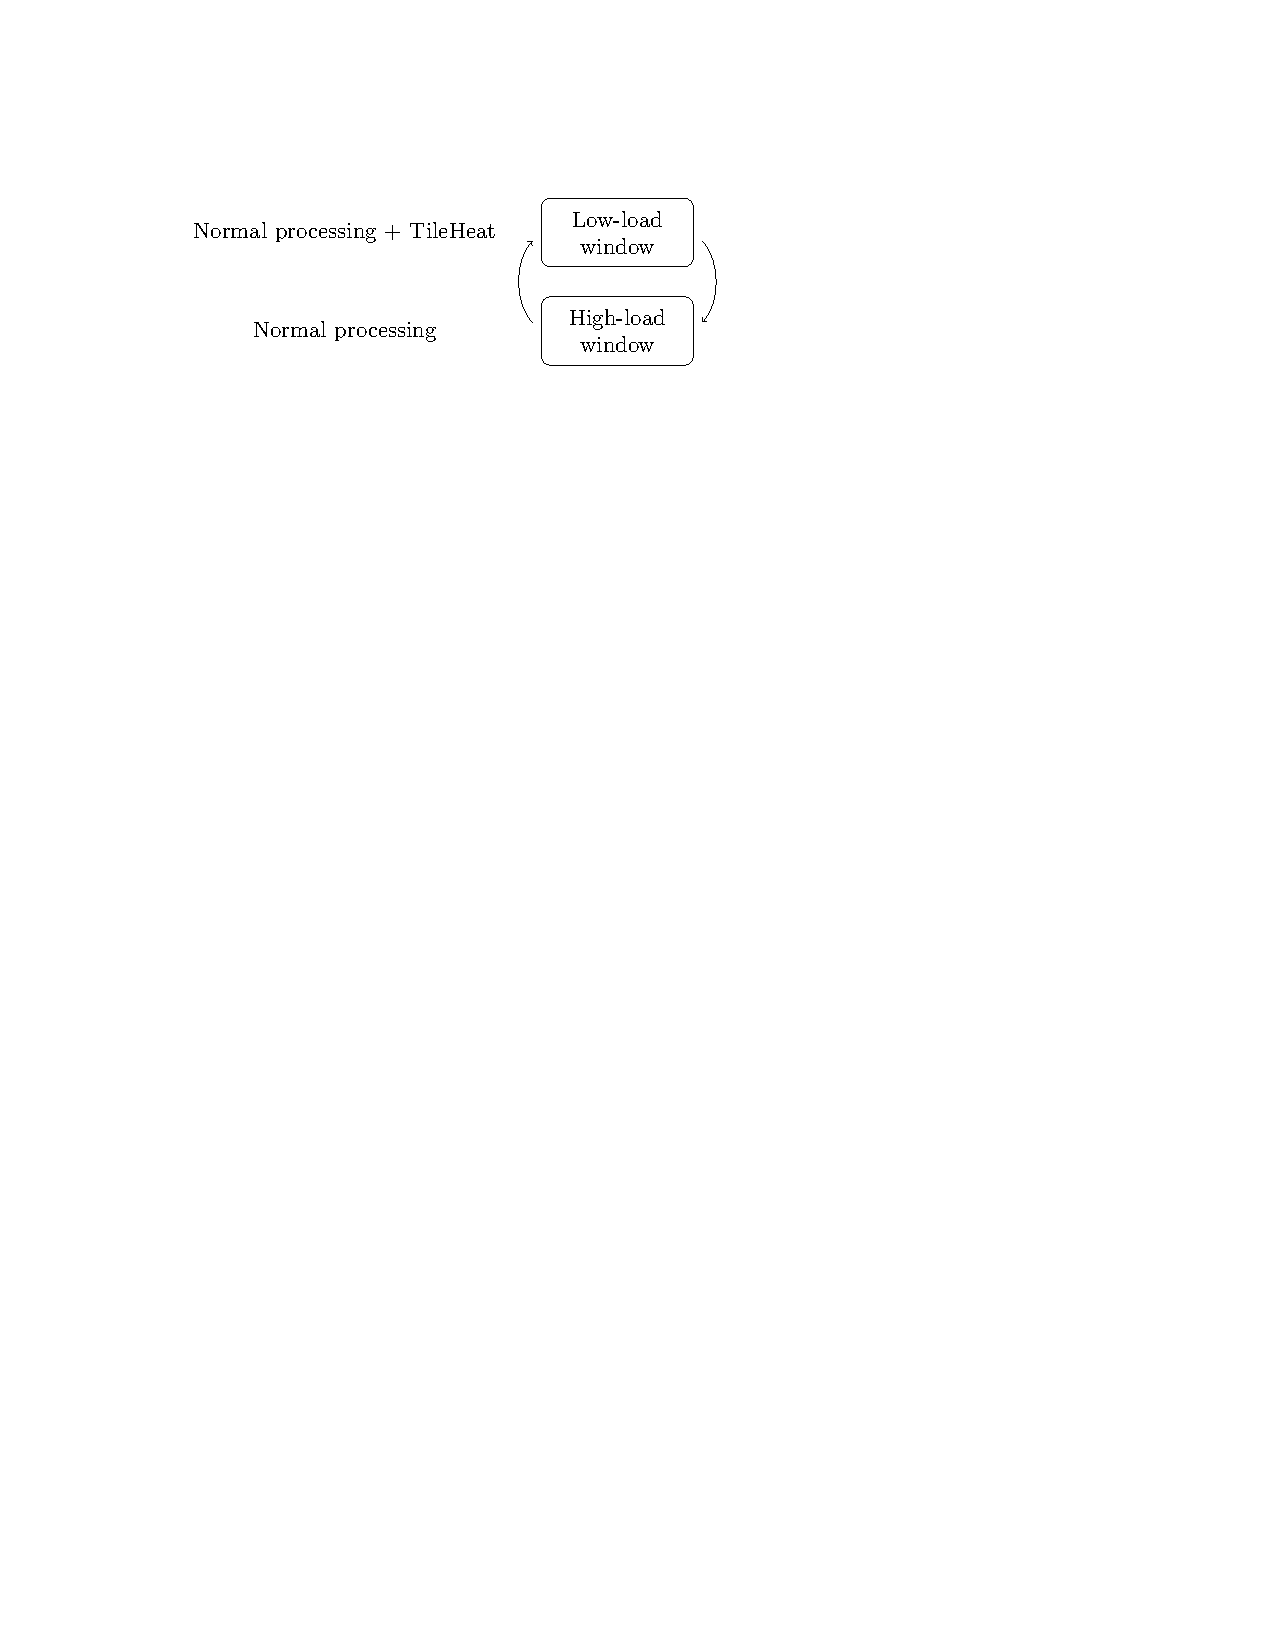
\includegraphics[scale=0.8]{figs-tileheat/figoverview}
\caption{Time periods and time windows: Processing during high- and low-load windows.}
\label{fig:high:low}
\end{figure}

%We assume that the base data from which the tiles are generated, gets updated frequently, which makes it a bad strategy to compute the entire set of tiles. 

\subsection{Tasks performed by TileHeat}
\label{sec:tileheat:tasks}

TileHeat is a framework for embedding tile selection algorithms into a log analysis procedure. The log analysis procedure computes a set of $n$ heatmaps, and passes these to tile selection. Tile selection in turn employs a \emph{prediction algorithm}, which predicts the heatmap for time $t + 1$. TileHeat uses the predicted heatmap to select which tiles to materialize for the next high-load window. 

The following steps are performed in time period $t+1$ by the TileHeat framework:
%
\begin{enumerate}
\item A prediction algorithm uses heatmaps for time periods $t-n$ to $t$ to predict the heatmap for time period $t+1$.
\item The tiles in the predicted heatmap are sorted in non-increasing order by heat.
\item The $k$ first tiles that are not already materialized are selected.
\item The materialization of the $k$ tiles is scheduled.
\end{enumerate}

The number $k$ is chosen as the number of tiles that can be materialized during the current low-load window. Various algorithms can be used to predict the heatmap for $t + 1$. In this work, we present two algorithms for the TileHeat framework: HEAT-HW (Section~\ref{sec:heat:hw}) and HEAT-D (Section~\ref{sec:heat:d}).

The running time of TileHeat can be estimated as follows. Let $m$ be the number of requests in the request log for time periods $t-n$ to $t$. We assume that the number of \texttt{GET} requests for each log request is bounded by a constant. The number of tile requests is therefore $O(m)$. By using a hash table, we can build the heatmaps in (expected) $O(m)$ time. As the sorting step takes at most $O(m)$ tiles as input, the (expected) running time of TileHeat is $O(m \log m)$ --- plus the running time of the prediction algorithm. 

\subsection{HEAT-HW algorithm}
\label{sec:heat:hw}
We have developed the HEAT-HW algorithm, which uses exponential smoothing applied to the heatmaps for time periods $t-n$ to $t$. Specifically, we use Holt-Winter double exponential smoothing~\cite{chatfield88}, which takes the trend of the observed variable into account. We motivate our choice of smoothing function in two ways:

\begin{enumerate}
\item We apply a smoothing function in general to avoid overfitting to the training data. Although the data we have analyzed is very stable, we introduce smoothing to prepare the algorithm for less stable workloads.
\item We use Holt-Winter smoothing in particular because it captures the trend in popularity for each tile. In future work, we would like to make use of the trend to adapt proactively to sudden rises in popularity for a geographical subregion by increasing the number of nodes serving those tiles. This of course implies a multi-node cache.
\end{enumerate}

Exponential smoothing is applied by treating each heat tile index $(i,j,z)$ as a separate variable. The equations for double exponential smoothing for heatmaps are given below (assuming that the first time period is $0$).

\begin{eqnarray*}
s_{i,j,z}^0 & = & h_{i,j,z}^0 \\
b_{i,j,z}^0 & = & h_{i,j,z}^1 - h_{i,j,z}^0 \\
s_{i,j,z}^{t+1} & = & \alpha h_{i,j,z}^0 + (1 - \alpha)(s_{i,j,z}^{t} + b_{i,j,z}^{t} ) \\
b_{i,j,z}^{t+1} & = & \beta (s_{i,j,z}^{t+1} - s_{i,j,z}^{t}) + (1 - \beta) b_{i,j,z}^{t}  \\
\end{eqnarray*}

As defined in Section~\ref{sec:heatmap:model}, $h_{i,j,z}^t$ is the observed heat of tile $(i,j,z)$ in time period $t$; $s_{i,j,z}^t$ is the smoothed value for time $t$ and $b_{i,j,z}^t$ is the trend for time $t$. Parameters $\alpha$ and $\beta$ are determined experimentally.

\subsection{HEAT-D algorithm}
\label{sec:heat:d}
The exponential smoothing as used in HEAT-HW only ranks tiles that are actually requested in the training data. Often, the training data is sparse, or tiles that are not accessed in the time periods $t-n$ to $t$ get accessed in time $t+1$, due to local changes in the spatial distribution of tile requests. 

HEAT-D is inspired by Tobler's first law of geography: ``Everything is related to everything else, but near things are more related than distant things''. HEAT-D works by applying a dissipation step to all heatmaps prior to applying Holt-Winter double exponential smoothing. The dissipation step is similar to the Jacobi method used for numerically solving the heat equation~\cite{templates}.

The following steps are performed by HEAT-D: 

\begin{enumerate}

\item For each heatmap of time periods $t-n$ to $t$, apply $p$ iterations of the dissipation step. An iteration consists of moving a fraction of the heat of each cell $(i,j,z)$ to its eight neighbors. This fraction is controlled by  a dissipation constant $\mu$. The corresponding differences in heat applied to each cell are shown in Figure~\ref{fig:dissipate}. 

\item Apply HEAT-HW over the heatmaps obtained in the step above. 

\end{enumerate}

%We apply $p$ rounds of the dissipation step to each heatmap in the training data. For each index $(i,j,z)$ in the heatmap, the dissipation step moves a fraction of the heat for that tile to its eight neighbors, based on a dissipation constant $\mu$. The process is illustrated in Figure~\ref{fig:dissipate}.

\begin{figure}
\centering
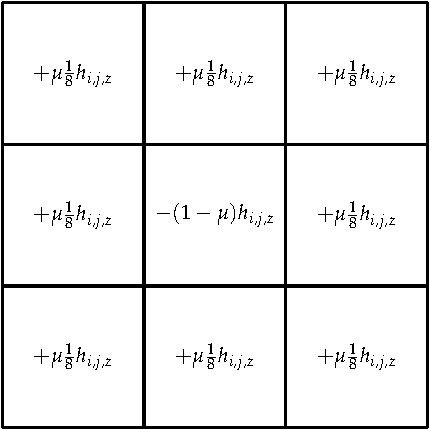
\includegraphics[scale=1]{figs-tileheat/disspate2}
\caption{Each dissipation step transfers heat from a center cell to each of it's eight neighbors. The center cell $(i,j,z)$ loses $(1 - \mu) h_{i,j,z}$ heat, and the neighbors gain $\mu \frac{1}{8} h_(i,j,z)$ heat. This is repeated for all center cells that are not on the border of the heatmap, using double buffering to avoid prematurely updating the heat of a cell.}
\label{fig:dissipate}
\end{figure}

The result of running dissipation on a sparse sample set can be seen in Figure~\ref{fig:dissipate_before_after}.

\begin{figure*}
\centering
\begin{tabular}{ll}
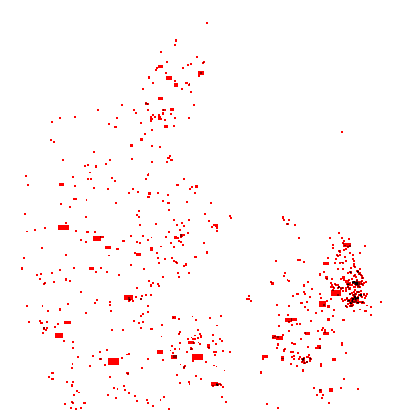
\includegraphics[scale=0.5]{figs-tileheat/heat_d-before.png} & 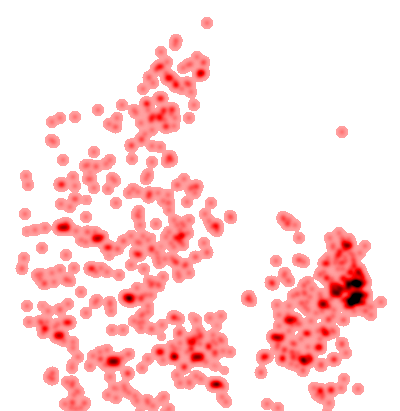
\includegraphics[scale=0.5]{figs-tileheat/heat_d-after.png} \\
\end{tabular}
\caption{Result of running the dissipation algorithm on a sparse heatmap (left) which contains $1.25\%$ of the samples used to create the heatmaps of Figure~\ref{fig:heatmaps}. The result (right) covers the hot regions of the heatmaps in Figure~\ref{fig:heatmaps} much better.}
\label{fig:dissipate_before_after}
\end{figure*}

\section{Experiments}
\label{sec:experiments}

The goal of our experiments is to show the improvements that can be gained by TileHeat in real production workloads. We first describe our experimental setup (Section~\ref{sec:setup}) and then present results (Section~\ref{sec:results}).  
%in a real production setting. We use real production workloads to test the hit ratio of the selected tile sets. 

\subsection{Experimental setup}
\label{sec:setup}

Here we describe how we have executed the experimental evaluation of our algorithms using a production request log extracted from KMS. Due to constraints in both time and access to the production system, we have not actually materialized the tiles selected by our methods, so we could not measure the effect this would have on latency in a production environment. Assuming, however, that serving tiles from cache is much more CPU- and I/O-efficient than computing on demand, we believe that the effect would be significant, given the high hit ratios we are able to achieve (Section~\ref{sec:results}). 

\subsubsection{Datasets}
\label{sec:datasets}
To validate the algorithms we have developed, we have extracted six datasets from the KMS request log for the last quarter of 2011. The method we used was to randomly select six weekdays, and for each of these days, select the $n$ previous weekdays to be used as training data. We use $n=3$. 

%Each dataset thus consists of the following:
%
%\begin{itemize}
%\item One weekday to use for validation.
%\item Three previous weekdays to use as training data. 
%\end{itemize}

The size of the log of requests for each weekday is substantial, with over 800,000 WMS requests per day, which we translate into \texttt{GET} requests. 

\subsubsection{Methodology}
\label{sec:methods}

This section describes our experimental methodology. The algorithms we have tested are:

\begin{itemize}

\item OPT: the optimal algorithm, which builds a heatmap of the workload used for the validation, and uses this heatmap to select the tiles. 

\item GEOM: the method currently employed by KMS, described in Section~\ref{sec:existing:methods}.

\item HEAT-HW: our heatmap method with Holt-Winter double exponential smoothing, described in Section~\ref{sec:heat:hw}. For HEAT-HW, the best set of parameters we could devise was $\alpha = 0.2$ and $\beta = 0.1$. 

\item HEAT-D: our heatmap method extended with dissipation, described in Section~\ref{sec:heat:d}. For HEAT-D, we set $\mu = 0.05$. The number of iterations $p$ is calibrated according to the resolution of the heatmap being dissipated. Given a scale factor $s$, we set $p = s \times (\text{\#rows}+\text{\#columns})/2$. The intuition is that heatmaps with higher resolution need more iterations of the dissipation step in order to cover enough geographical area. We set $s = 0.002$. 

\end{itemize}

The methodology we have developed to test the algorithms consists of playing back the production request log, both to train the algorithms, and to validate their performance. The outline of the method is as follows:

\begin{enumerate}
\item Pick a random day $t$.
\item Compute $n$ heatmaps for the $n$ consecutive days leading up to and including $t$.
\item Compute the actual heatmap for day $t+1$ from the data. 
\item Normalize the cells of the actual heatmap for day $t+1$ by the sum of heat for all cells. Now, each cell in the actual heatmap contains the fraction of the hit ratio contributed by the corresponding tile for day $t+1$. 
\item Calculate the tile ranking for the OPT algorithm by sorting tiles according to normalized heat contained in the actual heatmap.
\item For each of the other algorithms, obtain the corresponding tile ranking for day $t+1$, and measure the hit ratio by cumulating normalized heat from the actual heatmap.    
%\item The $n$ heatmaps are given as input to the algorithms GEOM, HEAT-HW, HEAT-D, and the output consists of the corresponding predictions of the heatmap for day $t+1$.
%\item Independently sort the cells of the two predicted heatmaps by decreasing heat, obtaining two lists of sorted cells.
%\item For each list, iterate over the cells, starting with the cell with highest heat. For each cell, look up the heat of the corresponding cell in the actual heatmap for day $t+1$, and plot these heat values cumulatively.
\end{enumerate}


Our results show averages of the hit ratios obtained by running the algorithms against each of the six datasets, recalling that a dataset consists of three days used to train the algorithms, and one day used to validate the performance of the algorithm.

\subsection{Results}
\label{sec:results}

\begin{figure*}
\centering
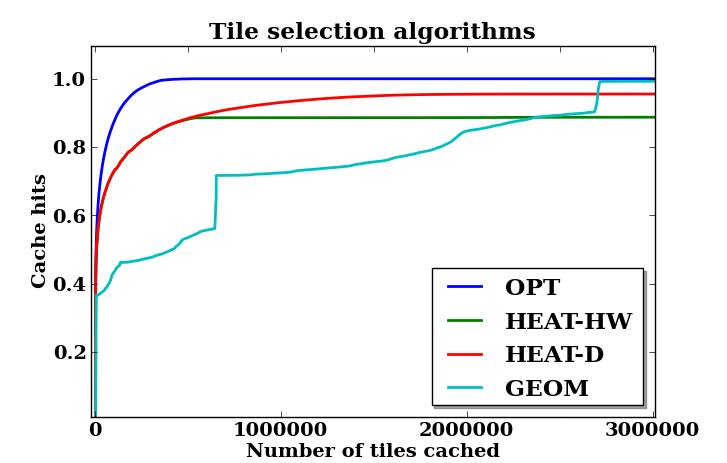
\includegraphics[scale=0.4]{figs-tileheat/results_closeup2.png}
\caption{The performance of tile selection algorithms for the first 3 million tiles selected, using three days of training data. The result is averaged over several runs using different data sets.}
\label{fig:results}
\end{figure*}

In Figure \ref{fig:results}, we show the average hit ratios obtained by the algorithms we have developed for TileHeat, using the datasets described in Section \ref{sec:datasets}. 
The figure shows the hit ratio of the first three million tiles that are selected by the algorithms. A full materialization contains more than ten million tiles. OPT, however, has a $100\%$ hit ratio after selecting 500,000 tiles. 

%OPT has a $100\%$ hit ratio after selecting 500,000 tiles.  %We also compare our algorithms against GEOM, which is the tile selection algorithm currently used by KMS.
As mentioned previously, the throughput of materializing tiles has been measured by KMS to be $58$ tiles per second on their infrastructure. A time window of $7.2$ hours fits inside the low load time period from $10$ PM to $6$ AM. During this window, we can compute $1.5$ million tiles. Within this tile budget, our best algorithm, HEAT-D, achieves a hit ratio of $95\%$. GEOM achieves a hit ratio of $76\%$ within the same tile budget. The hit ratio of HEAT-D is thus $25\%$ better than GEOM for this tile budget.

In general, we see that our algorithms rise significantly faster towards high hit ratios for small sets of tiles, e.g., in the 500,000 tile range. It is also clear that HEAT-D outperforms HEAT-HW after 500,000 tiles, and overall dominates HEAT-HW. This is because HEAT-D ranks more tiles than HEAT-HW, i.e., by ranking tiles that are not requested in the training workloads. We conclude that the additional tiles boost the hit ratio significantly, which confirms our hypothesis that tiles that are near to each other have similar access frequencies.

At around $2.6$ million tiles, GEOM overtakes HEAT-D, and becomes optimal. A peculiar effect of GEOM is a staircase effect that can be seen in Figure~\ref{fig:results}. We believe that this is an artifact of the way GEOM selects tiles --- selecting row-by-row the tiles that intersect the geometries provided. At certain latitudes, the rows cross over highly popular areas like the capital of Denmark, Copenhagen. The city of Copenhagen is clearly visible as a high-heat, dark area in the right side of each of the heatmaps shown in Figure~\ref{fig:heatmaps}. There are several steps in the staircase, as this effect is repeated at higher resolutions.

\section{Related work}
\label{sec:related}

Caching of dynamic web content has been extensively studied in a number of contexts~\cite{DDT+01:DynamicContentAcceleration,GMA+08:Ferdinand,GLR05:GoodEnough,LGZ04:MTCache,LKM+02:DBCache,Moh01:WebCaching}. A major issue investigated by these proposals is the policy used to keep the cache up-to-date. 
For example, Guo et al.~\cite{GLR05:GoodEnough} propose a set of declarative constraints that specify presence,  consistency, completeness, and currency of cached content. 
Garrod et al.~\cite{GMA+08:Ferdinand} explore how to take advantage of multiple cache servers while maintaining consistency. In contrast, our workload analysis shows that the main challenge for a geographical web service is the computational expense of the refresh procedure of the tile cache, rather than the freshness of relatively slowly updated map data. In this sense, our approach can be seen as similar to periodically refreshing a materialized view. This  ``view'' delivers the tile pyramid based on the underlying geographical data; however, it is both spatial and includes external user-defined functions to compute tile content. While similar in spirit to the materialized-view approach of MTCache~\cite{LGZ04:MTCache}, the additional complexities of our domain render the problem harder in several ways: First, not all of the view definition is available to the system, making it more difficult to predict which tiles are affected by which data and recompute selectively. Second, only portions of the view are of interest to end users, due to skew in access patterns, and it is not obvious how to define which portions are interesting ahead of time. Third, computation of tiles is a very resource-intensive user-defined function, making even a partial refresh of the spatial cache costly.  
 
Our work can also be seen as a self-tuning approach to managing a tile web cache~\cite{CN07:SelfTuning10YrPaper}. Similarly to online self-tuning approaches, such as COLT~\cite{SAMP07:COLT} and the seminal COMFORT~\cite{WHMZ94:COMFORT} project, TileHeat operates on a feedback loop, collecting workload characteristics, performing reasoning for choosing a new system configuration, and introducing configuration changes as necessary. However, our work differs in both the characterization of the problem as well as in the design choices we make for each step of our feedback loop. 
In particular, our choices are motivated by a careful analysis of the production log of a country-wide geographical web service. 
%We derive several conclusions from the analysis: 1) The access patterns of the rendering service exhibit high regularity, with low activity off day hours; 2) Access patterns can be largely inferred based on historical data, 3) The cost for materialization of tiles for caching is significant, and consequently services with moderate update rates -- such as geographical web services -- can dramatically profit from a selective cache.  

Adaptive algorithms have been studied for the classic buffer cache replacement problem, including 2Q~\cite{JS94:2Q}, ARC~\cite{MM03:ARC}, and LRU-K~\cite{OOW93:LRU-K}. Our work, however, is focused on the different scenario of spatial web caching, in which tiles are materialized in advance of processing the workload.
% Unlike previous caching algorithms, our approach takes advantage of the capability to observe the workload for a given time period, and uses the collected data to materialize a spatial cache for the next period.  
As in semantic caching~\cite{DFJ+96:SemanticCaching}, we exploit application characteristics to decide what data to cache and update. In contrast to semantic caching, we exploit spatial properties for higher web cache hit ratios, such as with our heat dissipation method. 
	
The basic idea of using heat to measure popularity of data items arises naturally in applications with skewed access patterns. For example, Scheuermann et al.~\cite{SWZ93:DiskCooling} propose schemes for data placement and adaptive load balancing that "cool" disks by redistributing file fragments. In spatial services more specifically, many researchers have observed that there is a strong skew in the access frequencies of tiles, and that this skew follows a power law~\cite{fisher07,LGXF12:SpatialPrefetching,talagala00}. Li et al.~\cite{LGXF12:SpatialPrefetching} exploit skew to create a pre-fetching model of spatial tiles, with focus on predicting short-term user navigation. Their work is based on a substantial body of related short-term prediction approaches~\cite{KKK01:Prefetching,KKK01:Prefetching2,LKK+02:Prefetching}. These methods are optimized for pre-fetching  tiles seconds before they are requested by a user. The amount of pre-fetching done during a time period is thus proportional to the load. As we have observed, load and latency are proportional, which means that pre-fetching in real time does little to alleviate load peaks. To reduce the high latency caused by load peaks, we instead pre-compute tiles during periods of low load. To achieve this, we develop methods that do not rely on the input of individual users browsing a map in real time. 
%In contrast, we look at the problem of pre-computing a large set of tiles that comprise a production-grade spatial web cache. 

As discussed in Section~\ref{sec:existing:methods}, Quinn and Gahegan~\cite{quinn10} suggest using certain classes of base objects, such as roads and coastlines, as predictors of where users will look at a map. However, as observed in Fisher's study of Microsoft Hotmap~\cite{fisher07}, real-world workloads can contradict models of rational user behavior, exclusively focused on a fixed set of rules. An example given by Fisher~\cite{fisher07} was a banner ad that caused frequent requests for ``empty'' parts of the Pacific Ocean. Based on such observations of real-life events, Fisher develops a multi-scale descriptive model that quantifies web map usage based on a heatmap. Their study supports our observation that anomalous patterns may be transient in time, but partially detectable from a training data set. In contrast to Fisher, however, we exploit this insight to propose multiple strategies to keep hit ratios on a spatial web cache high, while at the same time drastically reducing resource consumption during recomputation of tiles. 

\section{Conclusion}
% What we did
In this work, we propose and evaluate the use of heatmaps to analyze the request log for a geospatial service as well as to improve the creation time of a tile cache for this service. 
As we have observed, heatmaps can be made predictive and aid in selecting a set of high traffic tiles. We applied our techniques to the request log of a production system and showed that substantial improvements over an existing method were attained. In particular, using our HEAT-D algorithm to compute a tile cache yields a $25\%$ improvement in the hit ratio for a reasonable time window of materialization. HEAT-D accurately predicts the popularity of tiles that are not requested in the training data by employing a heat diffusion process. 

% Future work
While our results improve on existing methods, for future work we plan to do a more thorough exploration of the parameter space of the algorithms HEAT-HW and HEAT-D to investigate if further improvements could be achieved. In addition, we plan to work on efficient methods for materializing the tiles selected by our algorithms as well as use the trend information from HEAT-HW to build a distributed cache that adapts to sudden spikes in load. 
%Exploring efficient methods of materializing the tiles, given a plan computed by TileHeat, would bring the work full circle. 
Finally, deploying TileHeat in a production environment and measuring the effect on latency remains as an important direction of future work.

\section{Acknowledgements}
The authors would like to acknowledge the support of the National Survey \& Cadastre in Denmark and the Department of GIS \& IT at Grontmij Denmark, who have contributed economically, with data, and with human resources to this work.

% !TEX root = ./thesis.tex
\chapter{Conclusion}
\section{Summary}
\section{Future Work}

\bibliographystyle{plain}
\bibliography{thesis}
                             % Sample .bib file with references that match those in
                             % the 'Specifications Document (V1.5)' as well containing
                             % 'legacy' bibs and bibs with 'alternate codings'.
                             % Gerry Murray - March 2012



Marcos ambitious idea, three parts:
- (I) Introduction: talk about the two chapters that follow. 
- (P1) Pt 1: bulk: declarative cartography, about PRODUCING maps
- (P2) Pt 2: about SERVING digital maps
- Similar structure for both: state of the art, my contributions (advancing the state of the art).  

What-goes-where:
- I <- Case Study, P1 enables P2, Mention where related work is (which parts/chapters)
- P1 <- 
        Survey generalization, 
        CVL1 (closing the gap, part a), 
        CVL2 (closing the gap, part b)
- P2 <- 
        Survey on serving maps, getting to keyed data for maps, all this stuff you can use 
                incl. vectile (step 2),
                caching,
                prediction,
                data partitioning (step 3), 
                replication (step 4), 
                consistency, 
                key-value stores, 
                classic web serving infrastructures,
                papers from seminar
        Gap between state of the art, and the agency
        TileHeat (closing the gap, step 1), deploying a caching infrastructure
        
Publication strategy:

CVL2 (it's a journal thing, not a conference submission):
Approach: "Make CVL more general (star approach), with comparable performance"
- GeoInformatica (extended version of CVL), "completeness/thoroughness": repeat experiments, show new use cases (comp. to CVL), illustrate CVL2 with the new use cases 
- Only conference if "technical fun" or "something new" in compiler, real tech. take-away

\end{document}  

